\documentclass[
	12pt,				% tamanho da fonte
	openright,			% capítulos começam em pág ímpar (insere página vazia caso preciso)
	twoside,			% twoside para impressão em verso e anverso. Oposto a oneside
	a4paper,			% tamanho do papel. 
	% -- opções do pacote babel --
	english,			% idioma adicional para hifenização
	french,				% idioma adicional para hifenização
	spanish,			% idioma adicional para hifenização
	brazil				% o último idioma é o principal do documento
	]{abntex2}

% ---
% Pacotes básicos 
% ---
\usepackage{adjustbox}
\usepackage{amsmath}
\usepackage{mathtools}
\usepackage[printonlyused]{acronym}
\usepackage{lmodern}			% Usa a fonte Latin Modern			
%\usepackage{uarial}
%\renewcommand{\familydefault}{\sfdefault}
\usepackage[T1]{fontenc}		% Selecao de codigos de fonte.
\usepackage[utf8]{inputenc}		% Codificacao do documento (conversão automática dos acentos)
\usepackage{lastpage}			% Usado pela Ficha catalográfica
\usepackage{indentfirst}		% Indenta o primeiro parágrafo de cada seção.
\usepackage{color}				% Controle das cores
\usepackage{graphicx}			% Inclusão de gráficos
\usepackage{subcaption}
\usepackage{microtype} 			% para melhorias de justificação
\usepackage[brazilian,hyperpageref]{backref}	 % Paginas com as citações na bibl
\usepackage[alf]{abntex2cite}	% Citações padrão ABNT
\usepackage[table]{xcolor}
\usepackage{multirow}
\usepackage{pgfplots} %graficos
\usepackage{booktabs,makecell}
% ---

\usepackage{array}
\newcolumntype{L}[1]{>{\raggedright\let\newline\\\arraybackslash\hspace{0pt}}m{#1}}
\newcolumntype{C}[1]{>{\centering\let\newline\\\arraybackslash\hspace{0pt}}m{#1}}
\newcolumntype{R}[1]{>{\raggedleft\let\newline\\\arraybackslash\hspace{0pt}}m{#1}}
% --- 
% CONFIGURAÇÕES DE PACOTES
% --- 

\DeclareMathOperator*{\maxi}{Maximizar}
\DeclareMathOperator*{\mini}{Minimizar }

\newcommand{\icol}[1]{% inline column vector
  \left(\begin{smallmatrix}#1\end{smallmatrix}\right)%
}

% ---
% Configurações do pacote backref
% Usado sem a opção hyperpageref de backref
\renewcommand{\backrefpagesname}{Citado na(s) página(s):~}
% Texto padrão antes do número das páginas
\renewcommand{\backref}{}
% Define os textos da citação
\renewcommand*{\backrefalt}[4]{
	\ifcase #1 %
		Nenhuma citação no texto.%
	\or
		Citado na página #2.%
	\else
		Citado #1 vezes nas páginas #2.%
	\fi}%
% ---
% ---
% Informações de dados para CAPA e FOLHA DE ROSTO
% ---
% \titulo{Análise de Sentimentos baseada em emoções Aplicada as Redes Sociais}
\titulo{An\'{a}lise de Sentimentos Baseada em L\'{e}xicos na Detec\c{c}\~{a}o de \textit{Haters} Aplicada as Redes Sociais}
% \title{Análise de Sentimentos baseada em emoções Aplicada as Redes Sociais}
\title{An\'{a}lise de Sentimentos Baseada em L\'{e}xicos na Detec\c{c}\~{a}o de \textit{Haters} Aplicada as Redes Sociais
}
\autor{Álisson Rodrigues Teles}
\local{Caxias do Sul}
\data{2018}
\orientador{Carine G. Webber}
\coorientador{}
\universidade{UNIVERSIDADE DE CAXIAS DO SUL}
\instituicao{%
UNIVERSIDADE DE CAXIAS DO SUL
\par
ÁREA DO CONHECIMENTO DE CIÊNCIAS EXATAS E ENGENHARIAS
\par
BACHARELADO EM CIÊNCIA DA COMPUTAÇÃO}

\tipotrabalho{Projeto de Diplomação}
% O preambulo deve conter o tipo do trabalho, o objetivo, 
% o nome da instituição e a área de concentração 
\preambulo{Projeto de Diplomação submetido ao curso de Bacharelado em
Ciência da Computação do Centro de Computação e Tecnologia da
Informação da Universidade de Caxias do Sul, como requisito obrigatório para graduação.}
% ---

% alterando o aspecto da cor azul
\definecolor{blue}{RGB}{41,5,195}

% informações do PDF
\makeatletter
\hypersetup{
     	%pagebackref=true,
		pdftitle={\@title}, 
		pdfauthor={\@author},
    	pdfsubject={\imprimirpreambulo},
	    pdfcreator={LaTeX with abnTeX2},
		pdfkeywords={abnt}{latex}{abntex}{abntex2}{trabalho acadêmico}, 
		colorlinks=true,       		% false: boxed links; true: colored links
    	linkcolor=blue,          	% color of internal links
    	citecolor=blue,        		% color of links to bibliography
    	filecolor=magenta,      		% color of file links
		urlcolor=blue,
		bookmarksdepth=4
}
\makeatother
% --- 

% --- 
% Espaçamentos entre linhas e parágrafos 
% --- 

% O tamanho do parágrafo é dado por:
\setlength{\parindent}{1.3cm}

% Controle do espaçamento entre um parágrafo e outro:
\setlength{\parskip}{0.2cm}  % tente também \onelineskip

% ---
% compila o indice
% ---
\makeindex
% ---

% ----
% Início do documento
% ----
\begin{document}

% Retira espaço extra obsoleto entre as frases.
\frenchspacing 

% ----------------------------------------------------------
% ELEMENTOS PRÉ-TEXTUAIS
% ----------------------------------------------------------
% \pretextual

% ---
% Capa
% ---
\imprimircapa
% ---

% ---
% Folha de rosto
% (o * indica que haverá a ficha bibliográfica)
% ---
\imprimirfolhaderosto*
% ---

% ---
% Inserir a ficha bibliografica
% ---
%% Isto é um exemplo de Ficha Catalográfica, ou ``Dados internacionais de
% catalogação-na-publicação''. Você pode utilizar este modelo como referência. 
% Porém, provavelmente a biblioteca da sua universidade lhe fornecerá um PDF
% com a ficha catalográfica definitiva após a defesa do trabalho. Quando estiver
% com o documento, salve-o como PDF no diretório do seu projeto e substitua todo
% o conteúdo de implementação deste arquivo pelo comando abaixo:
%
% \begin{fichacatalografica}
%     \includepdf{fig_ficha_catalografica.pdf}
% \end{fichacatalografica}
\begin{fichacatalografica}
	\vspace*{\fill}					% Posição vertical
	\hrule							% Linha horizontal
	\begin{center}					% Minipage Centralizado
	\begin{minipage}[c]{12.5cm}		% Largura
	
	\imprimirautor
	
	\hspace{0.5cm} \imprimirtitulo  / \imprimirautor. --
	\imprimirlocal, \imprimirdata-
	
	\hspace{0.5cm} \pageref{LastPage} p. : il. (algumas color.), 30 cm.\\
	
	\hspace{0.5cm} \imprimirorientadorRotulo~\imprimirorientador\\
	
	\hspace{0.5cm}
	\parbox[t]{\textwidth}{\imprimirtipotrabalho~--~\imprimirinstituicao,
	\imprimirdata.}\\
	
	\hspace{0.5cm}
		1. AMQP.
		2. \textit{Analytic Hierarchy Process}.
		I. André Luis Martinotto.
		II. Universidade de Caxias do Sul.
		III. Faculdade de Ciências da Computação.
		IV. Avaliação de intermediadores de mensagem que implementam o protocolo \textit{AMQP}\\ 			
	
	\hspace{8.75cm} CDU 02:141:005.7\\
	
	\end{minipage}
	\end{center}
	\hrule
\end{fichacatalografica}
% ---

% ---
% Inserir folha de aprovação
% ---
% Isto é um exemplo de Folha de aprovação, elemento obrigatório da NBR
% 14724/2011 (seção 4.2.1.3). Você pode utilizar este modelo até a aprovação
% do trabalho. Após isso, substitua todo o conteúdo deste arquivo por uma
% imagem da página assinada pela banca com o comando abaixo:
%
% \includepdf{folhadeaprovacao_final.pdf}
%
\begin{folhadeaprovacao}

  \begin{center}
    {\ABNTEXchapterfont\large\imprimirautor}

    \vspace*{\fill}\vspace*{\fill}
    \begin{center}
      \ABNTEXchapterfont\bfseries\Large\imprimirtitulo
    \end{center}
    \vspace*{\fill}
    
    \hspace{.45\textwidth}
    \begin{minipage}{.5\textwidth}
        \imprimirpreambulo
    \end{minipage}%
    \vspace*{\fill}
   \end{center}
        
   Trabalho aprovado. \imprimirlocal, 13 de dezembro de 2018: 

   \assinatura{\textbf{\imprimirorientador} \\ Orientador} 
   \assinatura{\textbf{Daniel Luís Notari} \\ Convidado 1}
   \assinatura{\textbf{Helena Graziottin Ribeiro} \\ Convidado 2}
   \begin{center}
    \vspace*{0.5cm}
    {\large\imprimirlocal}
    \par
    {\large\imprimirdata}
    \vspace*{1cm}
  \end{center}
  
\end{folhadeaprovacao}
% ---

% ---
% Dedicatória
% ---
%\include{diversos/dedicatoria}
% ---

% ---
% Agradecimentos
% ---
%\include{diversos/agradecimentos}
% ---

% ---
% RESUMOS
% ---
%% resumo em português
\setlength{\absparsep}{18pt} % ajusta o espaçamento dos parágrafos do resumo
\begin{resumo}

As redes sociais estão cada vez mais inseridas no cotidiano das pessoas. Essas ferramentas trazem melhoria na comunicação e disseminação de opiniões, permitindo que várias culturas se unam em meio a postagens sobre os mais variados assuntos. Os brasileiros estão cada vez mais inseridos nos meios tecnológicos e são ativos usuários dessas redes sociais. Contudo, com a liberdade de expressão vieram comportamentos agressivos de preconceito, os discursos de ódio, tendo como alvos mulheres, deficientes, negros e muçulmanos, espalhando ódio e assédios verbais. O controle sobre postagens violentas e de assédio moral é normalmente realizado de forma manual. O uso de ferramentas automatizadas pode auxiliar e facilitar esta tarefa. Com base nisso, o trabalho pretende abordar a Análise de Sentimentos aplicada às redes sociais para detectar discursos de ódio de raça, gênero, religião, e deficiência, especificamente na língua portuguesa. Este tema é relevante já que poucos trabalhos têm abordado a Análise de Sentimentos e geração de base de léxicos para o idioma português. Ao longo deste trabalho pretende-se gerar um dicionário léxico, contendo termos da língua portuguesa, para uso na detecção de \textit{haters}. Tal léxico será usado em um software específico, que uma vez integrado ao \textit{Twitter}, será testado e avaliado.
%Os resultados obtidos serão comparados com uma aplicação de Redes Neurais Artificiais empregada com o mesmo propósito de classificação.

 \textbf{Palavras-chaves}: Análise de Sentimentos, Discurso de Ódio, Twitter, Haters, Weka
\end{resumo}

% resumo em inglês
\begin{resumo}[Abstract]
 \begin{otherlanguage*}{english}
   Social networks are increasingly inserted in people's daily lives. These tools bring improvement in communication and dissemination of opinions, allowing multiple cultures to come together amid postings on the most varied subjects. Brazilians are increasingly inserted in the technological media and are active users of these social networks. However, with freedom of expression came aggressive behavior of prejudice, hate speech, targeting women, disabled, blacks and Muslims, spreading hatred and verbal harassment. Control over violent posting and bullying is usually done manually. The use of automated tools can help and facilitate this task. Based on this, the work intends to approach the sentiment analysis applied to social networks to detect hate speech of race, gender, religion, and disability, specifically in the Portuguese language. This topic is relevant since few studies have dealt with the sentiment analysis and generation of a base of lexicons for the Portuguese language. Throughout this work we intend to generate a lexical dictionary, containing terms of the Portuguese language, for use in the detection of haters. This lexicon will be used in a specific software, which once integrated with Twitter, will be tested and evaluated.

   \vspace{\onelineskip}
 
   \noindent 
   \textbf{Keywords}: Sentiment Analysis, Hate Speech, Twitter, Haters, Weka
 \end{otherlanguage*}
\end{resumo}

% ---

% ---
% inserir lista de ilustrações
% ---
\pdfbookmark[0]{\listfigurename}{lof}
\listoffigures*
\cleardoublepage
% ---

% ---
% inserir lista de tabelas
% ---
\pdfbookmark[0]{\listtablename}{lot}
\listoftables*
\cleardoublepage
% ---

% ---
% inserir lista de abreviaturas e siglas
% ---
\begin{siglas}
   \item[ATE]{\textit{Automatic Term Expansion}}
   \item[CURE]{\textit{Clustering Using Representatives}}
   \item[DNA]{\textit{Deoxyribonucleic acid}}
   \item[DWT]{\textit{Discrete Wavelet Transform}}
   \item[EM]{\textit{Expectation-Maximization Clustering}}
   \item[HGKA]{\textit{Hibrid Genetic k-means Algorithm}}
   \item[MUSA]{\textit{Motif Finding Using na Unsupervised Approach}}
   \item[TCC]{\textit{Trabalho de Conclusão de Curso}}
\end{siglas}
% ---
% inserir o sumario
% ---
\pdfbookmark[0]{\contentsname}{toc}
\tableofcontents*
\cleardoublepage
% ---

% ----------------------------------------------------------
% ELEMENTOS TEXTUAIS
% ----------------------------------------------------------
\textual

\chapter{Introdução}
\label{cap:Introducao}
% contextualizar 
Com a globalização do uso da \textit{internet}, a sociedade aprimorou a sua forma de interagir e desenvolveu novas ferramentas para as relações interpessoais, profissionais e etc. Essas ferramentas são chamadas de redes sociais e são exemplos o \textit{Facebook}\footnote{\url{https://www.facebook.com}}, o \textit{Twitter}\footnote{\url{https://twitter.com}} e o \textit{Instagram}\footnote{\url{https://www.instagram.com}} entre outros no mercado. Essas ferramentas estão presentes na maioria dos \textit{smartphones} da população, e a cada dia aumentam o número de usuários ativos em suas plataformas. Segundo pesquisa realizada pelo \citeonline{ibge2018}, $64,7\%$ das pessoas de 10 anos ou mais utilizaram a \textit{internet} e $94,6\%$ das conexões foram realizadas por \textit{smartphones}. Ainda na mesma pesquisa foi verificado que $94,2\%$ da finalidade dessas conexões foi enviar ou receber mensagens de texto, áudio ou imagens por aplicativos diferentes de \textit{e-mail}. Dentro dessas inúmeras publicações existem muitos conteúdos que são de interesse comum da população já que a mesma está compartilhando seu conhecimento, crítica e opinião aumentando a participação nos mais variados assuntos, desde opinião sobre determinado produto até descontentamento social, há também riscos de agressão verbal entre os membros das comunidades e, o gerenciamento manual acaba sendo impossível devido ao número de dados gerados a cada dia.

% falar sobre o desafio na área 
Para realizar a análise textual dessa imensa quantidade de dados é necessário o uso de recursos computacionais já que a análise manual se torna impraticável  pela demora no tempo de resposta. O número crescente de opiniões também gerou o interesse de grandes empresas em garimpar grupos públicos em interpretar os sentimentos manifestados de seus usuários para verificar aprovação de seus produtos sem necessitar de pesquisas pessoais e até invasivas, diminuindo gastos e acelerando as conclusões para tomadas de decisões. Além disso, há uma necessidade de ferramentas que realizem a análise tendo como base a língua portuguesa já que existem poucas com resultados satisfatórios e poucas pesquisas relacionadas ao idioma.

% apresentar solução
É Nesse contexto que se desenvolve a técnica de \textit{Sentiment Analysis}, uma subárea da TDM (\textit{Text Data Mining})\cite{Hearst:1999:UTD:1034678.1034679}, que se refere ao processo de extrair padrões (conhecimentos de interesse das mais variadas áreas de pesquisa) de documentos textuais não estruturados tendo enfase na detecção das emoções envolvidas nessas produções que podem ter seus sentimentos classificados em: positivos, negativos e neutros. \cite{Li:2010:SAG:2898607.2898826}. 

%bebefícios na area 
As vantagens em fazer pesquisa de opinião por meio de \textit{Sentiment Analysis} são: o baixo custo de análise, rapidez de pesquisa e resposta, autenticidade e não invasão. Sendo os últimos dois itens os maiores diferenciais da técnica pelo fato de as informações usadas como objeto de estudo serem buscadas de comunidades públicas e de a veracidade das informações ser natural já que os usuários não são previamente avisados sobre a pesquisa a ser realizada. Trazendo avanços para a indústria, órgãos públicos, e até mesmo para o indivíduo essa é uma área de pesquisa em crescimento sendo também crescente o interesse em ferramentas ágeis para resultados em tempo real. 

A mesma liberdade de expressão que a \textit{internet} proporcionou deu lugar para que pessoas também utilizem as redes sociais para propagar discursos de ódio contra grupos de minoria. Tornando a \textit{internet} também um lugar hostil com agressões verbais \cite{Chetty2018}.  Além disso, poucos trabalhos abordaram o tema contextualizando o problema na língua portuguesa tornando esse um tema distante e silencioso.

\section{Objetivos}
\subsection{Objetivo Geral}    
    Esse trabalho tem por objetivo desenvolver e avaliar um \textit{software} de detecção de \textit{haters} baseado em Análise de Sentimentos expressos em textos na Língua Portuguesa. 

\subsection{Objetivos Específicos}
    Para atingir o objetivo geral serão seguidos os seguintes objetivos específicos:
\begin{enumerate}
    \item Identificar métodos computacionais para a Análise de Sentimentos e detecção de \textit{haters}.
    \item Implementar um método para detecção de \textit{haters} em dados textuais.
    \item Realizar testes do \textit{software} desenvolvido, comparando os resultados com análises feitas por especialistas humanos.
    \item Avaliar o desempenho do método implementado.
\end{enumerate}
	
\section{Organização do Documento}
O restante do trabalho é organizado da seguinte maneira:

\begin{itemize}

\item \textbf{Capítulo \ref{cap:REFERENCIAL} - Revisão Bibliográfica:} Compreende toda a fundamentação teórica necessária para o desenvolvimento e entendimento do estudo apresentado. É apresentado as etapas principais desenvolvidas em uma análise de sentimento, bem como os principais algoritmos utilizados na classificação dos textos, uma breve explicação dos conceitos de redes sociais, além de estudo de discurso de ódio dentro dessas plataformas. Alguns trabalhos relacionados também são citados no final do capítulo.

\item \textbf{Capítulo \ref{cap:Desenvolvimento} - Desenvolvimento:} São apresentadas as etapas previstas, bem como a metodologia utilizada no desenvolvimento do trabalho tendo o objetivo de criar uma base de léxicos contidos em discursos de ódio, a integração com \textit{software} já desenvolvido que realiza Análise de Sentimentos baseado em emoções e a verificação da efetividade nas detecções de discursos de ódio.

\item \textbf{Capítulo \ref{cap:conclusoes} - Conclusões:} É apresentada síntese do trabalho desenvolvido até então, bem como projeção de atividade futuras em cronograma de atividades detalhado no final do capítulo.
\end{itemize}

% ----------------------------------------------------------
% REFERENCIAIS TEORICOS
% ----------------------------------------------------------
%\part{Referenciais teóricos}
\chapter{Análise de Sentimentos}
\label{cap:REFERENCIAL}

A Análise de Sentimentos, ou ainda mineração de opiniões, é uma subárea da mineração de textos que analisa atitudes e emoções expressas de forma textual. Segundo \citeonline{BAHRI2018669}, a Análise de Sentimentos tem por objetivo a classificação de um dado textual baseado no seu teor sentimental, de opinião, de avaliação e de atitudes, sendo útil na avaliação de determinadas entidades que podem ser eventos, produtos, problemas, entre outros. 

Tendo em vista o crescimento do número de usuários nas redes sociais, consequentemente o número de produções textuais nesses canais aumentou. Em razão disso, o interesse de grandes empresas em obter pesquisas de opinião a partir de publicações em redes sociais, ficou evidente. A Análise de Sentimentos, quando realizada de forma manual por especialistas, é inviável, sendo necessário o uso de recursos computacionais unidos a algoritmos sofisticados realizando análises em grande escala (\textit{big data}) em menor tempo \cite{BAHRI2018669}.
% falar sobre a procura pelas

\section{Etapas da Análise de Sentimentos}

O processo de Análise de Sentimentos compreende diversas etapas para que, de forma automática, dados textuais sejam avaliados em termos de sentimentos expressos neles. O processo é composto pelas etapas que são descritas nas seções seguintes: coleta de dados, pré-processamento dos dados, classificação dos dados.  

\subsection{Coleta de Dados}
\label{subsec:coletadados}
A primeira fase para a mineração de opinião é a coleta de dados que serão posteriormente processados. Segundo \citeonline{9788576089346}, "Dados são fatos coletados e normalmente armazenados. Informação é o dado analisado e com algum significado. O conhecimento é a informação interpretada, entendida e aplicada para um fim.". O trabalho considerará dados eletrônicos digitais, mais precisamente, dados não estruturados (postagens textuais) gerados em redes sociais de forma manual. A informação principal considerada será a análise léxica baseada em categorias de emoções. Já o conhecimento pretendido será a aplicação estatística em cima das informações obtidas.

Para a fase de coleta de dados é importante primeiramente definir qual será a fonte de dados e, após, desenvolver ferramentas automáticas para a coleta dos dados que se pretende analisar futuramente. Algumas redes sociais disponibilizam APIs (\textit{Application Programming Interface}) para que aplicações sejam desenvolvidas usando o banco de dados dessas plataformas, permitindo tanto o consumo como a geração de dados dentro delas por meio de postagens de fotos, vídeos, textos. Essas ferramentas conseguem realizar buscas com filtros de data, usuários, palavras-chave, e etc. Sendo possível buscar amostras específicas conforme o que se queira pesquisar.

Geralmente as APIs são \textit{web services} (produtos disponibilizados na \textit{internet}) baseados no protocolo HTTP (\textit{Hypertext Transfer Protocol}) e tornam os acessos seguros por meio da geração de \textit{tokens} a cada nova solicitação de inserção, alteração ou exclusão de dados. Um exemplo é a \textit{Graph API}\footnote{\url{https://developers.facebook.com/docs/graph-api}} desenvolvida pelo \textit{Facebook}, ela disponibiliza uma interface gráfica chamada \textit{Graph API Explorer} que pode ser vista na figura \ref{fig:GraphAPIExplorer}. A ferramenta é gratuita e tutoriais são disponibilizados para a aprendizagem.

\begin{figure}[!h]
\centering 
\caption{Tela do \textit{Graph API explorer}}
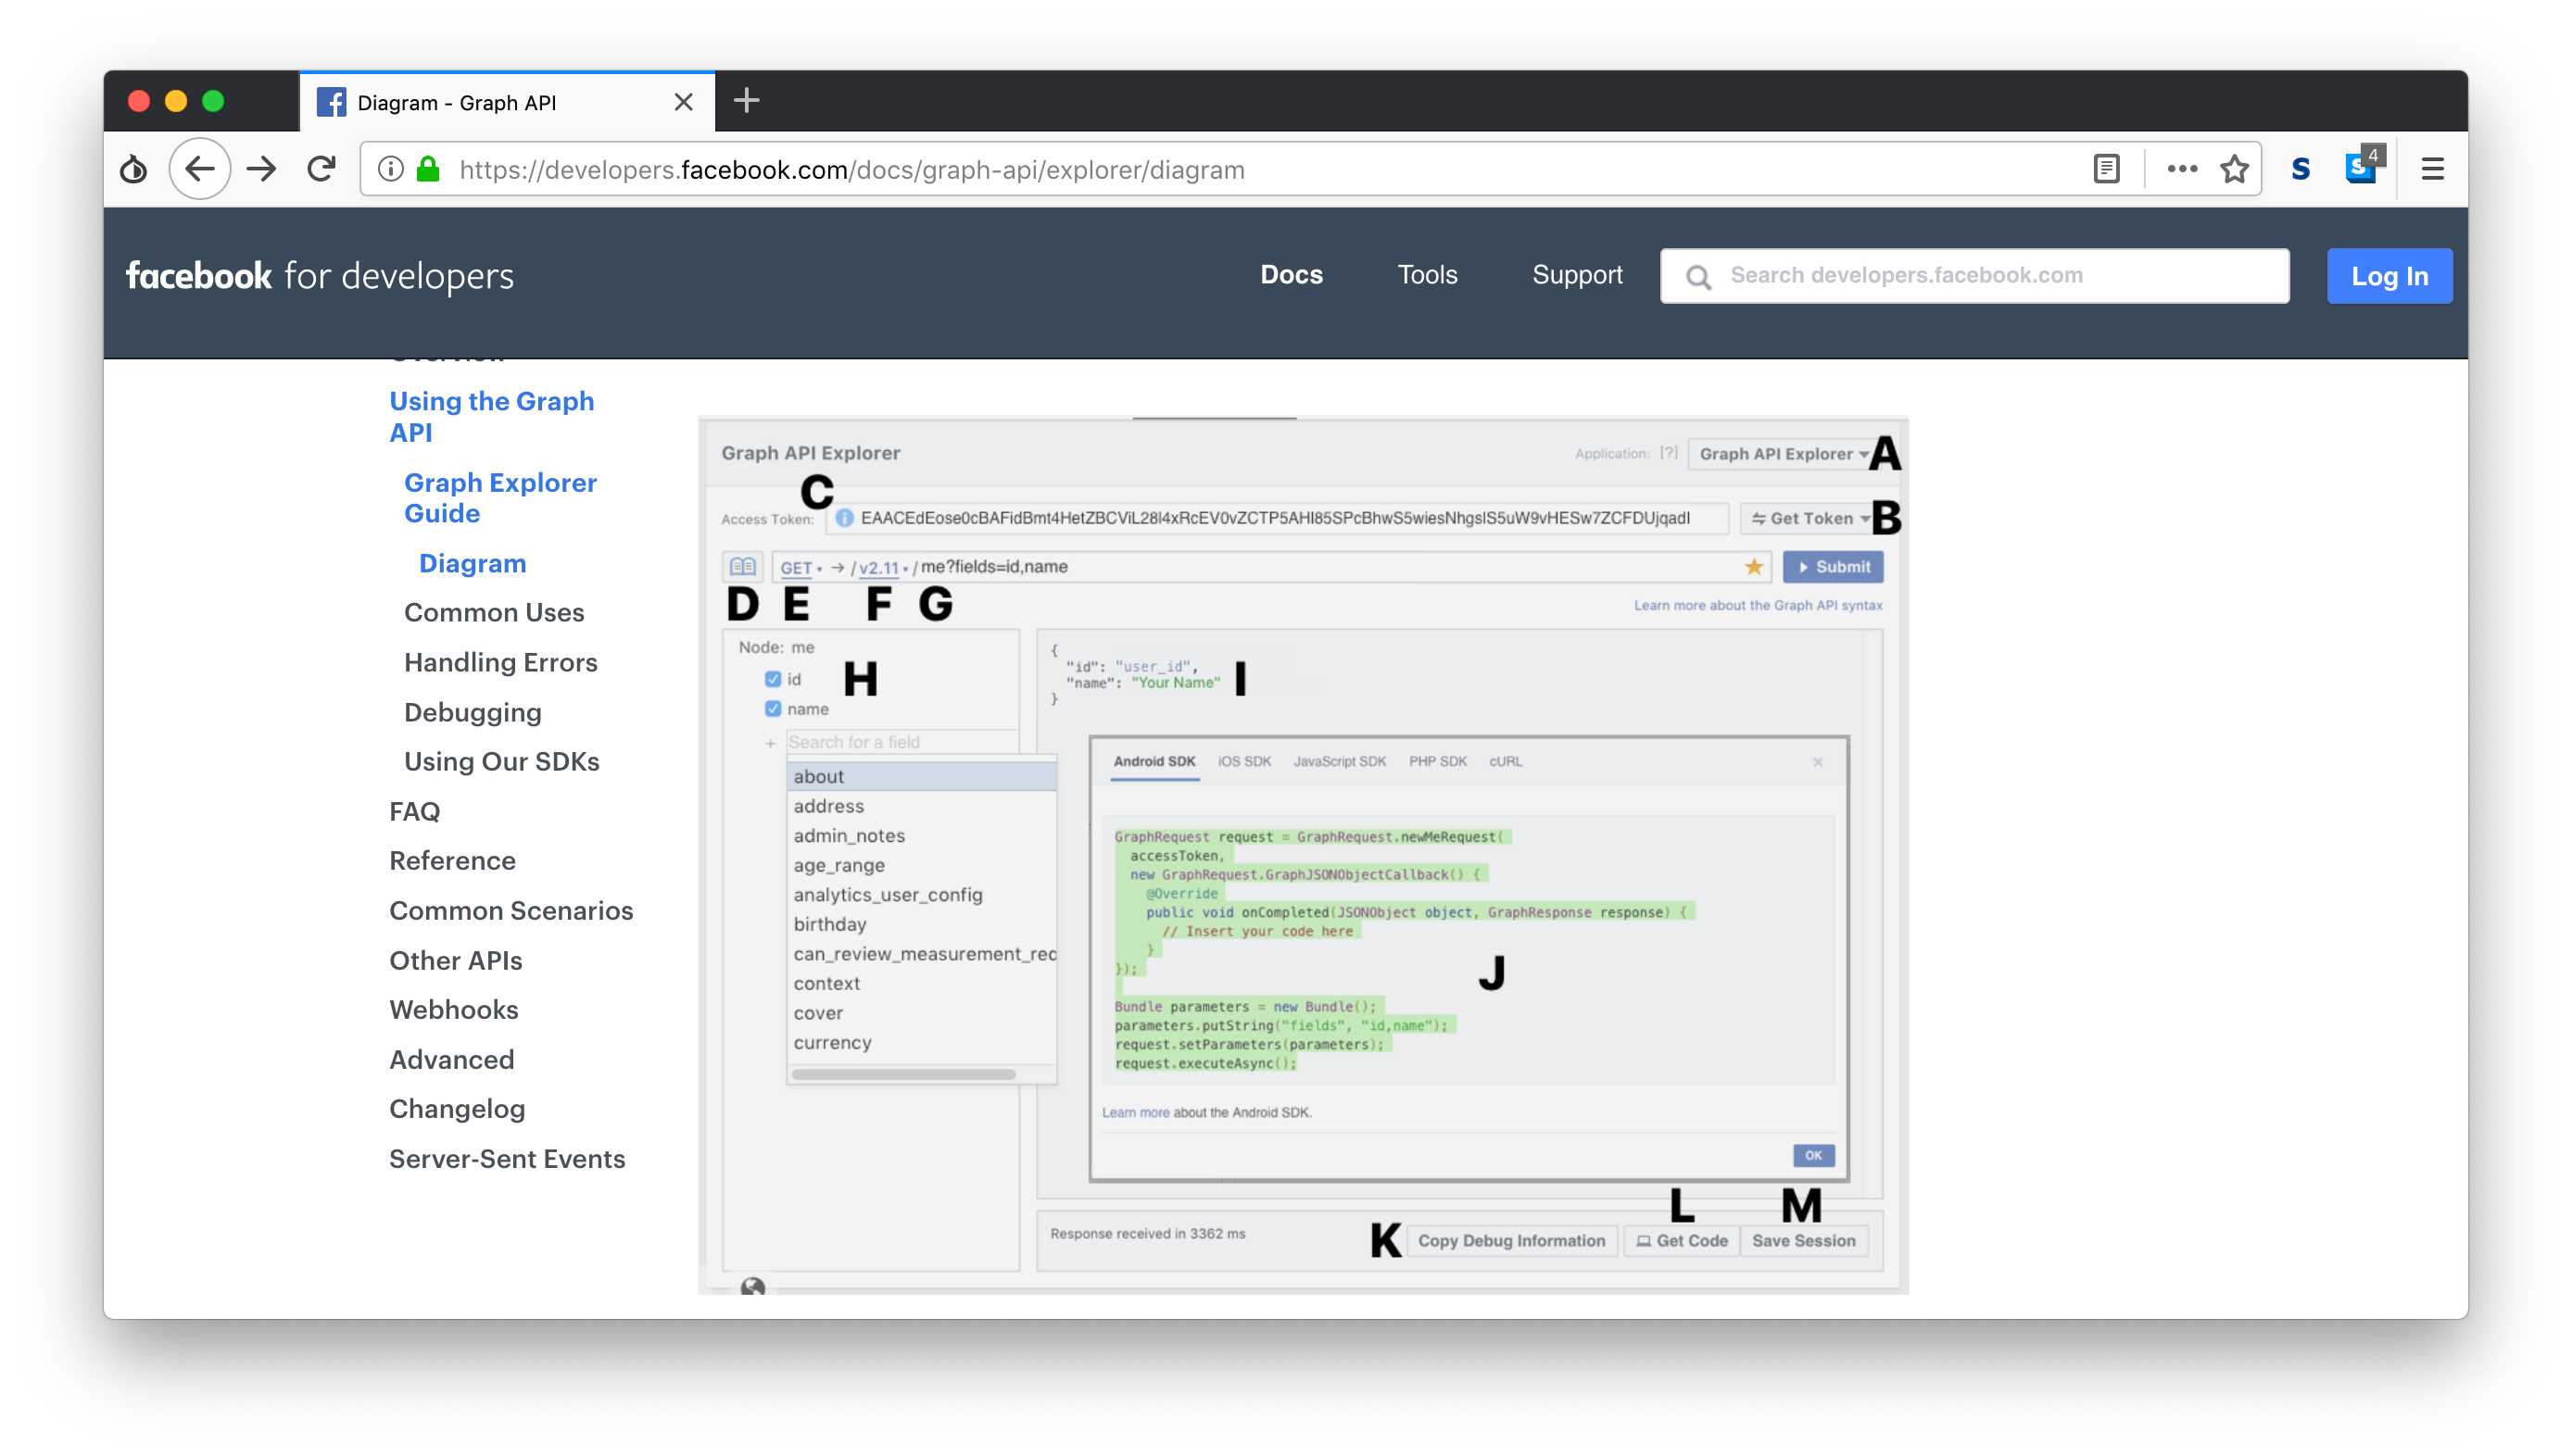
\includegraphics[scale=0.35]{imagens/graphapiexplorer.png}
\legend{Fonte: (FACEBOOK, 2018)}
\label{fig:GraphAPIExplorer}
\end{figure}

\subsection{Pré-processamento dos Dados}
\label{subsec:preproc}

Após a coleta e armazenagem dos dados, é necessário a remoção de informações desnecessárias, a padronização do formato dos dados obtidos e a apresentação dos dados que serão, posteriormente, processados pelos algoritmos de extração de conhecimento. O pré-processamento inicia com a separação das frases em listas de palavras agora chamadas de \textit{tokens} que serão processadas até transformar o conteúdo inicial em sua forma reduzida e otimizada \cite{SYMEONIDIS2018298}. É importante considerar que as técnicas de pré-processamento são utilizadas conforme a fonte de dados e também dos termos de interesse que serão buscados, assim como o idioma dos textos que se quer analisar. 

A seguir serão apresentadas as principais técnicas de pré-processamento textual conforme levantado pelos autores \citeonline{SYMEONIDIS2018298}, sendo apresentadas em ordem de importância para um melhor resultado, tendo ganho de performance já que é possível a execução em paralelo entre as combinações de algumas técnicas. Também são citados alguns trabalhos que tratam cada uma das técnicas descritas:

\begin{itemize}
\item Remoção de \textit{unicode} e ruídos: Como nem todos os \textit{datasets} tem um tratamento prévio disponibilizado pelas ferramentas de coleta, é necessário um primeiro tratamento do seu conteúdo. Essa tarefa consiste em remover códigos \textit{unicode}\footnote{ Padrão internacional de códigos que permite que qualquer computador seja capaz de interpretar qualquer sistema de escrita \cite{0321480910}.} indesejados   como "\textbackslash u002c" e "\textbackslash x06". Essa é a primeira tarefa e também o ponto de partida para as demais tarefas de pré-processamento \cite{SYMEONIDIS2018298}.

\item Substituição de \textit{URL} e menções de usuários: A maioria dos conteúdos textuais em redes sociais contém URLs, menções de usuário e \textit{tags} (sendo chamadas no \textit{Twitter} de \textit{hashtag}). Como esses conteúdos não apresentam nenhum conteúdo semântico e não expressam nenhum sentimento, essa etapa tem por objetivo a remoção total ou substituição por um \textit{token} universal dentro do universo possível \cite{Khan2014}.
\label{it:giria}

\item Substituição de abreviaturas e gírias: Os usuários de redes sociais escrevem em linguagem coloquial e é comum o uso de gírias e de abreviação. Nessa etapa é gerada, manualmente, uma lista com as principais abreviaturas e expressões que se deseja detectar e também os termos que devem substituir essas frases. Assim, sempre que alguma frase especificada na lista for detectada, imediatamente será substituída pela frase equivalente \cite{Kouloumpis}.

\item Remoção de conteúdo numérico: Nessa etapa qualquer conteúdo numérico será removido pois eles não tem nenhum sentimento expresso. é importante a execução dessa etapa logo após a execução da tarefa anterior, (substituição de abreviaturas e gírias) pois muitas gírias são compostas por números e a sua substituição já elimina a necessidade de remoção dos números \cite{He:2011:AEP:2002472.2002489}.

\item Substituição de pontuação repetida: Em muitos casos os usuários das redes sociais usam pontuações sendo eles de interrogação, de exclamação e de parada (ponto final) quando usados repetidamente significam sentimento intenso. Nessa etapa quando essas pontuações forem encontradas mais de uma vez em sequência as mesmas poderão ser substituídas por uma \textit{token} de mesmo valor em sentimento.

\item Remoção de pontuações: Sendo uma técnica muito comum na mineração de texto, essa consiste em remover as pontuações presentes no texto. Muitas literaturas afirmam que uma pontuação exclamativa pode significar um sentimento intenso positivo ou negativo e que sua remoção pode também alterar a acurácia da classificação do texto \cite{Lin2009}.

\item Manipulação de palavras em caixa alta: Palavras escritas em caixa alta são consideradas intensas de emoção. Por isso antes de padronizar todas as letras que compõem o texto para letras minúsculas, as palavras, com mais de duas letras, que forem escritas em caixa alta serão detectadas e sinalizadas para posterior processamento dos algoritmos de classificação .

\item Padronização de letras minúsculas: É a etapa mais comum verificada nas literaturas relacionas ao pré-processamento de texto. A etapa tem por objetivo a substituição de todos os caracteres maiúsculos para minúsculos, padronizando o conteúdo e facilitando as próximas etapas de pré-processamento \cite{DBLP:conf/coling/SantosG14}.

\item Remoção de \textit{stopwords}: Por definição, \textit{stopwords} são palavras de baixo peso e desnecessárias na Análise de Sentimento dos textos, são palavras com alta frequência de apresentação.  As \textit{stopwords} são adicionadas a listas chamadas por \textit{stoplists} previamente definidas conforme a necessidade da aplicação, podendo ser alterada a qualquer momento. Nessa etapa todas as palavras contidas na \textit{stoplist} serão removidas do texto já que não tem nenhuma utilidade na Análise de Sentimentos.

\item Substituição de palavras alongadas: As palavras alongadas são palavras escritas incorretamente com a repetição de algumas letras, escritas assim propositalmente para salientar sentimentos do autor. Nessa etapa as palavras alongadas serão encurtadas para sua forma original, perdendo parte do sentimento atribuído já que ocorrem com pouca frequência dentro de um mesmo texto \cite{Mohammad2015}.

\item Correção ortográfica: É comum em textos informais a presença de palavras com erros ortográficos. Nessa etapa é sugerido que, com o auxílio de dicionários externos ocorra uma correção ortográfica das palavras. Após a correção ortográfica a Análise de Sentimentos se torna mais simples já que as palavras incorretas trazem uma enorme dificuldade na classificação de sentimento das mesmas.

\item \textit{Part-of-Speech} (POS): Na etapa de POS, ou ainda, marcação de parte da fala, algumas classes de palavras são desconsideradas por não terem sentimentos atribuídos como advérbios, verbos, e etc. Na maioria dos estudos na área de pré-processamento de textos são considerados verbos, advérbios e substantivos, pois esses podem ser considerados na classificação \cite{Barbosa:2010:RSD:1944566.1944571}.

\item Lematização: Talvez uma das etapas mais complexas apresentadas nesse trabalho, tem por objetivo a busca dos lemas das palavras, isto é, fazer a análise morfológica das palavras em busca da remoção dos lexemas. Muitas literaturas não usam essa etapa pois a mesma é complexa e seu uso pode impactar na performance do pré-processamento \cite{Guzman2014}.

\item \textit{Stemming}: consiste na separação das palavras em \textit{radical} + \textit{terminação} para a análise apenas do radical das mesmas. Esse procedimento pode resultar em maior peso para o termo em posterior análise \cite{Porter1980}.
\end{itemize}

Após o pré-processamento, os dados estarão mais consistentes e padronizados, contendo as informações mais relevantes para a avaliação do conhecimento. Existem algumas tratativas específicas para \textit{emojis} e símbolos que também demonstram sentimento. Os mesmos não serão abordados no trabalho por ser de baixa relevância na pesquisa.

\subsection{Classificação dos Dados}
Após o pré-processamento, a próxima etapa da Análise de Sentimentos é a classificação dos dados. Atualmente existem vários estudos que buscam encontrar os métodos mais eficientes para a classificação, podendo ser visto na Figura \ref{fig:SAMethods} as principais abordagens para a etapa de classificação dos dados. Os algoritmos de \textit{machine learning} trazem um grande avanço na assertividade dos resultados da Análise de Sentimentos. Tradicionalmente os algoritmos de classificação de Análise de Sentimentos atribuem um sentimento como "positivo", "negativo" e "neutro", existindo algumas abordagens baseadas em análise de emoção que consideram categorias mais amplas baseadas no estudo de \citeonline{Ekman1992} que podem ser: alegria, tristeza, raiva, medo, nojo e surpresa.  

A seguir serão apresentados os principais métodos abordados nas literaturas referenciais que são os métodos baseados em léxico e os baseados em  aprendizado de máquina (\textit{machine learning}).

\begin{figure}[!h]
\centering 
\caption{Métodos de classificação de Análise de Sentimentos}
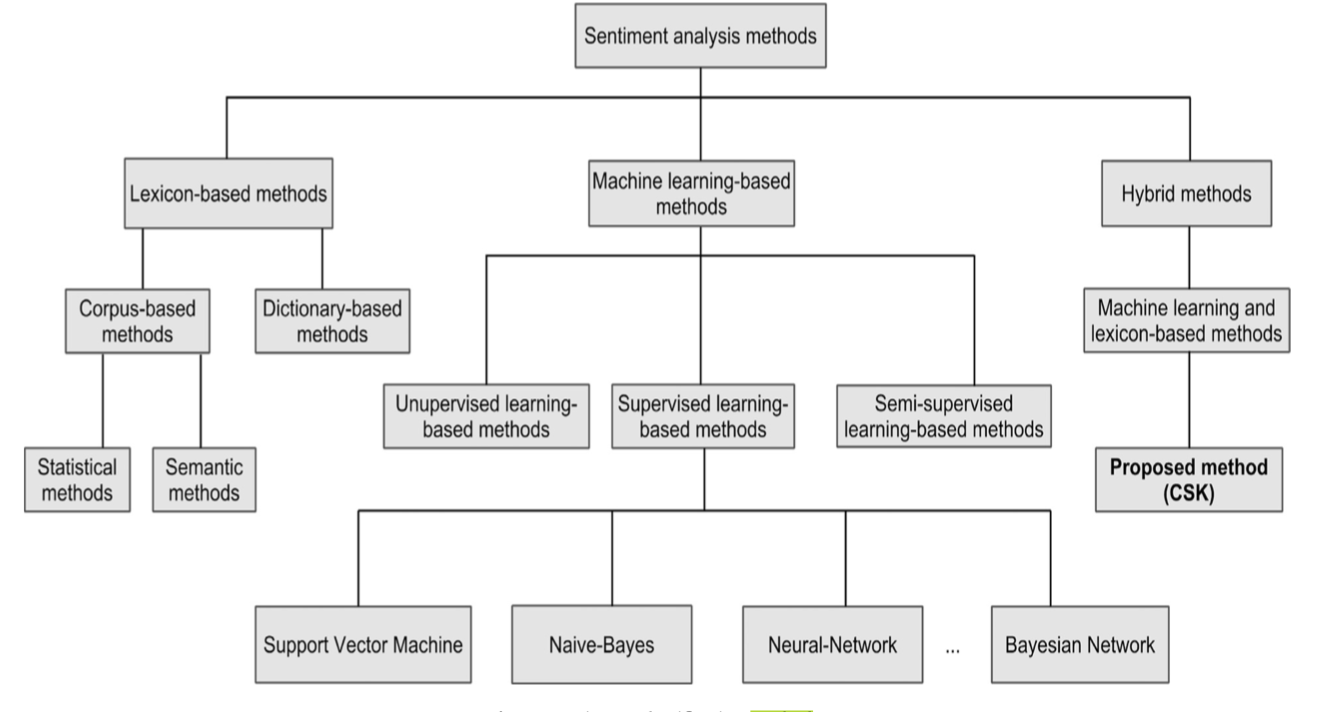
\includegraphics[scale=0.70]{imagens/sentimentanalysismethods.png}
\legend{Fonte: \cite{CHANDRAPANDEY2017764}}
\label{fig:SAMethods}
\end{figure}
\newpage

\subsubsection{Método Baseado em Aprendizado de Máquina}

Nessa abordagem a classificação dos dados ocorre com o auxilio de algoritmos de \textit{machine learning} como rede neural, algoritmo \textit{Naive-Bayes}, \textit{K-mean}s e etc, podendo ser um algoritmo supervisionado, ou ainda, não-supervisionado. A seguir uma descrição e exemplos de cada abordagem.

\subsubsubsection{Métodos Supervisionados}

Segundo \citeonline{TRUYENS2014153}, são métodos supervisionados todos aqueles que usam exemplos fornecidos por especialistas humanos de domínio para ensinar o algoritmo a interpretar informações linguísticas interpretativas, ou seja, são algoritmos que tem uma fase de aprendizado \textit{a priori} de executar a classificação. Ainda segundo os autores, os algoritmos supervisionados geram resultados significantes porém, têm um algo custo devido ao esforço humano necessário. Mesmo assim, algumas práticas semi-supervisionadas, usando uma pequena base de dados rotulados e conjunto a uma base maior não rotulada relacionadas por suposição (por exemplo, pela distribuição uniforme dos dados) os resultados são realmente satisfatórios \cite{TRUYENS2014153}.

O principal algoritmo supervisionado utilizado dentro da classificação de sentimentos é o \textit{Naive Bayes} (NB) por unir simplicidade e eficiência nos cenários mais diversos, especialmente quando aplicado a um conjunto de dados onde seus atributos são independentes \cite{VIEGAS2018153}. 

O Naive Bayes é um algoritmo probabilístico baseado no Teorema de Bayes representado na Equação \ref{eq:naivebayes}. Ela é definida como "a probabilidade de A dado B", ou seja, qual a probabilidade de A estar dentro de um conjunto de evidências assumido como B \cite{schmitt2013analise}.

\begin{equation}
    \label{eq:naivebayes}
     P\left ( A| B \right ) = \frac{P\left ( B|A \right )P\left ( A \right )}{P\left ( B \right )}
\end{equation}

O algoritmo é considerado ingênuo (\textit{naive}) por assumir que cada atributo é independente, ou seja, a informação de um evento não é informativa sobre nenhum outro. A Figura \ref{fig:ModeloNaiveBayes}  indica que cada atributo $A_{i}$ influência a classe $C$ unicamente sem nenhum atributo influenciar qualquer outro \cite{schmitt2013analise}.

\begin{figure}[!h]
\centering 
\caption{Modelo \textit{Naive Bayes}}
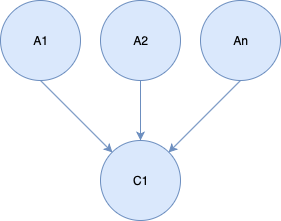
\includegraphics[scale=0.70]{imagens/modeloNaiveBayes.png}
\legend{Fonte: O autor baseado em \cite{schmitt2013analise}}
\label{fig:ModeloNaiveBayes}
\end{figure}

O algoritmo pode ser usado de forma incremental conforme a necessidade de sua revisão probabilística. Existem várias abordagens de modelo sendo os principais o modelo binário e o modelo multidimensional. No modelo binário, cada documento é representado por um vetor binário onde a a presença ou a ausência de um termo é representado, respectivamente, por $1$ e $0$. Já no modelo multidimensional a representação ocorre por vetores de números inteiros por documento, onde  cada índice do vetor representa a quantidade de vezes que um termo acontece no documento \cite{schmitt2013analise}.

\subsubsubsection {Métodos Não-Supervisionados} 

São tidos como métodos não-supervisionados aqueles que o próprio algoritmo - sem o auxilio de aprendizado a partir de treinamento - determina as características do texto. Um exemplo é a clusterização de textos onde o \textit{software} analisa um conteúdo textual encontrando, independentemente, grupos de palavras com similaridade entre elas. Essa abordagem é baseada em três etapas principais: a medida de proximidade, estratégia de agrupamento e seleção de descritores.

Na etapa de medida de proximidade verifica-se a similaridade entre os textos, dependendo da abordagem também é válido buscar a dissimilaridade entre os textos. Os dois métodos mais conhecidos para a obtenção dessa medida de proximidade para dados do tipo texto são os métodos: Cosseno e \textit{Jaccard}. Para a execução de ambos os métodos é necessário considerar dois vetores documentos $x_{i}=\left ( x_{i1}, x_{i2}, \dotsc, x_{im}\right )$ e $x_{j}=\left ( x_{j1}, x_{j2}, \dotsc, x_{jm}\right )$ onde cada termo da coleção é representado em uma das dimensões dos vetores \cite{Rezende2011}.

O método do cosseno, expresso na Fórmula \ref{eq:cosseno}, define a semelhança dos termos conforme o ângulo que os vetores formam entre si. Para ângulos próximos de $90^{\circ}$, ou seja, cosseno próximo de 0, os documentos não compartilham nenhum termo. Já para ângulos próximos de $0^{\circ}$, e  cosseno próximo de 1, os documentos têm termos semelhantes \cite{Rezende2011}.

\begin{equation}
    \label{eq:cosseno}
     \cos \left ( x_{i},x_{j} \right ) = \frac{\sum_{l=1}^{m} x_{il} x_{jl}}{\sqrt{\sum_{l=1}^{m} x_{il^{2}} \sum_{l=1}^{m} x_{jl^{2}}} }
\end{equation}

Para as situações em que os vetores são representados por valores binários, indicando presença ou ausência de determinados termos, o cálculo de proximidade pode ser realizado pelo método \textit{Jaccard} \cite{Rezende2011}.

Para o cálculo considera-se os mesmos vetores $x_{i}$ e $x_{j}$  considerando também as seguintes contagens:

$f_{01}$: Número de termos ausentes em $x_{i}$ e presentes em $x_{j}$;

$f_{10}$: Número de termos presentes em $x_{i}$ e ausentes em $x_{j}$;

$f_{11}$: Número de termos presentes em ambos os vetores.

Com essas medidas, a medida \textit{jaccard} é dada conforme a Fórmula \ref{eq:jaccard}. O resultado estará compreendido entre $\left [ 0,1 \right ]$ sendo que quanto mais próximo de $1$, maior a similaridade dos termos.

\begin{equation}
    \label{eq:jaccard}
     jaccard(x_{i},x_{j}) = \frac{f_{11} }{f_{10} +f_{01}  + f_{11} }
\end{equation}

Após encontrar as medidas de similaridade é necessário  realizar a etapa de agrupamento sendo o \textit{k-means} um dos modos mais utilizados onde o objetivo é agrupar os vetores em $k$ grupos. A seguir são apresentadas as características do \textit{k-means} conforme  \citeonline{Steinbach00acomparison}.

O \textit{k-means} é baseado na ideia de que um ponto central pode representar um \textit{cluster}, e nessa técnica se usa a noção de centroide que significa o ponto médio central de um grupo de pontos. Geralmente o centroide é um ponto diferente de um ponto de dados real e é calculado a partir dos demais vetores do grupo \cite{Steinbach00acomparison}. A fórmula do centroide para um vetor de tamanho $G$, onde $x$ é um vetor documento, é dada a seguir:

\begin{equation}
    \label{eq:centroide}
     C=\frac{1}{|G|}\sum_{x \in G}x
\end{equation}

Como entrada do algoritmo \textit{k-means} tem-se um conjunto de vetores documento e $k$, que é o número referente a quantidade de grupos que se deseja se dividam. A partir daí o algoritmo selecionará $k$ vetores aleatórios como centroides iniciais e repetir o cálculo de dissimilaridade de cada vetor para cada centroide e inserir o documento no grupo no qual ele mais se assemelha. Após, uma nova centroide será calculada tendo em vista os vetores que foram adicionados a ele. O algoritmo pode assumir duas regras de parada: na primeira, é considerado o número de iterações e na segunda é considerado, a situação onde não ocorrem mais alterações nos vetores, ou seja, os vetores não trocam mais de grupos \cite{Steinbach00acomparison}.

A última etapa dos métodos não-supervisionados é a seleção de descritores para apresentação dos resultados para a próxima etapa da Análise de Sentimentos. Alguns métodos para a seleção de descritores utilizam o centroide, já que ele mantém a característica central de todos os grupos.

\subsubsection{Método Baseado em Léxico}
\label{subsubsec:lexico}
No método baseado em léxico o sentimento (polaridade) é calculado conforme sua orientação semântica. É necessário definir um dicionário léxico com as polaridades correspondentes de cada palavra que o compõe. Esses dicionários podem ser criados manualmente ou automaticamente usando radicais de palavras e as adicionando a lista conforme apresentado por \citeonline{Taboada}. Primeiro uma lista de adjetivos e suas polaridades correspondentes é desenvolvida e um dicionário é criado. Após, quando um texto for analisado todos os seus adjetivos serão extraídos e arquivados junto de seus valores que podem no final gerar uma polaridade única do texto analisado \cite{Taboada}. Existem duas subclasses principais dentro da abordagem léxica que são: as técnicas de Análise de Sentimento baseadas em dicionário e as técnicas de Análise de Sentimento baseada em corpo \cite{LIU2017149}.

Na AS baseada em dicionário o foco principal da técnica é a construção de dicionários de sentimento, onde um pequeno conjunto de palavras e sentimentos é determinado manualmente e após ocorre uma pesquisa dos antônimos e sinônimos nas corporas mais populares como o \textit{WordNet} \cite{Miller:1995:WLD:219717.219748}, \textit{HowNet}, ou ainda \textit{Thesaurus}, fazendo com que novas palavras sejam encontradas e o dicionário aumente consideravelmente. O processo iterativo da técnica é realizado até que nenhuma nova palavra possa ser encontrada, resultando em um dicionário de sentimentos \cite{LIU2017149}. 

Já na AS baseada em corpo é comumente utilizada quando se quer encontrar padrões sintáticos de contextos específicos. O foco da técnica é encontrar os padrões sintáticos e uma lista de radicais, comumente chamados de sementes, de palavras de opinião. Para chegar ao resultado, a técnica usa técnicas estatísticas para encontrar as palavras sementes enquanto as técnicas semânticas são utilizadas para determinar os valores semânticos para as palavras conforme a similaridade, conforme as diferentes palavras \cite{LIU2017149}.

\section{Redes Sociais}
\label{sec:RedesSociais}
Desde o princípio, a humanidade tem a necessidade de conviver em comunidade, sendo necessário a vida em conjunto na realização de trabalhos como também para a formação de famílias e grupos. Esses grupos eram formados conforme afinidades políticas, religiosas, étnicas, profissionais e etc, trazendo como resultado o constante desenvolvimento social e e intelectual do homem até os dias atuais \cite{KHALED2018}. Com o desenvolvimento da \textit{internet} esse comportamento também foi replicado para a rede em plataformas denominadas \textit{Online Social Network} (OSN), também chamadas de Redes Sociais, que segundo \citeonline{N2018777} vão além de plataformas de comunicação e troca de informações, mas também chegam a impactar no crescimento econômico. 

São exemplos de redes sociais o \textit{Facebook}\footnote{\url{https://www.facebook.com}}, o \textit{Twitter}\footnote{\url{https://twitter.com}} e o \textit{Instagram}\footnote{\url{https://www.instagram.com}} sendo todos baseados na cocriação com o usuário, isto é, ele que gera o conteúdo das plataformas através dos seus \textit{posts}, as conexões através das solicitações de conexão com outro usuário, comunidades através de páginas de afinidade e grupos, e sinaliza possíveis melhorias para as plataformas seguirem em contínua evolução atraindo mais usuários a cada ano, como pode ser visto na Tabela \ref{tab:qtdusers} a quantidade de usuários em Agosto de 2018 nas redes sociais.


\begin{table}[h]
\centering
\caption{Quantidade de usuários nas redes sociais}
\label{tab:qtdusers}
\begin{tabular}{|l|c|}
\hline
\textbf{Rede Social}&  \textbf{Número de Usuários} \\ \hline
Facebook     &     2.23 bilhões   \\ \hline
Youtube      &     1.9  bilhão    \\ \hline
Instagram    &     1    bilhão    \\ \hline
Twitter      &     336  milhões   \\ \hline
Reddit       &     330  milhões    \\ \hline
Pinterest    &     200  milhões    \\ \hline
Ask.fm       &     160  milhões    \\ \hline
\end{tabular}
\legend{Fonte: \cite{kallas_2018}}
\end{table}

Existem redes sociais com o foco em conteúdo visual, que é o caso do \textit{Instagram}, rede social fundada em 6 de Outubro de 2010 por Kevin Systrom (CEO e co-fundador) e Mike Krieger (CTO e co-fundador) que revolucionou a forma de compartilhar fotos. Segundo Kevin Systrom, o \textit{Instagram} se tornou o lar das narrativas visuais, sendo possível que artistas, músicos, celebridades e qualquer tipo de pessoa compartilhe seus conteúdos \cite{instagram_2018}. A rede social conta com mais de 400 milhões de novas postagens na categoria de \textit{Story} diariamente. 

Também é o caso do \textit{Snapchat}, em que a companhia se intitula como uma \textit{empresa de câmeras} e que acredita que a revolução da sua ferramenta contribui com a forma das pessoas se expressarem, aprenderem sobre o mundo e se divertirem juntas \cite{snapchat_2018}. No \textit{Snapchat} as pessoas podem compartilhar momentos instantâneos por meio de foto ou vídeo, fazendo edições rápidas e casuais podendo também temporizar o tempo de exibição das postagens conforme necessitar.

O foco do trabalho desenvolvido é em redes sociais com conteúdo textual, como é o exemplo do \textit{Facebook} e o \textit{Twitter}, já que serão utilizados os métodos de pré-processamento abordados na Sub-sessão \ref{subsec:preproc} afim de melhorar a detecção de sentimentos. Dessa forma redes sociais com conteúdo de imagem como é caso do \textit{Instagram} podem ser avaliadas por trabalhos futuros com outras abordagens de pré-processamento e detecção de sentimentos.

\section{Discurso de Ódio nas Redes Sociais}
Como foi visto na Sessão \ref{sec:RedesSociais}, é cada vez maior a quantidade de informações geradas diariamente dentro das redes sociais. É também inquestionável a liberdade que as redes sociais trazem para seus usuários que podem expressar suas opiniões sobre os mais variados assuntos já que as plataformas permitem o compartilhamento de ideias entre usuários e entre comunidades de assuntos em comum. 

A liberdade de expressão acaba sendo necessária para que se mantenha os direitos (democráticos) dos indivíduos, proporcionando a troca de opiniões e o prazer autônomo. A mesma liberdade de expressão pode ser uma das causas da ocorrência de discursos de ódio sendo então eles  considerados descendentes da própria liberdade de expressão \cite{Chetty2018}.

Expressar o discurso de ódio tornou-se tendência pois o mesmo resulta em popularidade instantânea. O discurso de ódio viola os direitos fundamentais de um ser humano sendo que o objetivo mais amplo da liberdade de expressão é alcançar a auto-realização e estabelecer um equilíbrio aceitável entre estabilidade e mudanças sociais, sendo possível por meio da comunicação livre \cite{Chetty2018}.

O discurso de ódio pode prejudicar as vitimas de forma direta ou de forma indireta. Quando prejudica diretamente, as vítimas são imediatamente feridas pelo conteúdo do discurso. Já no discurso indireto de ódio, o dano pode ser imediato ou não, o dano retardado é gerado pelos agentes e não por um ator principal \cite{Seglow2016}. 

A Figura \ref{fig:atividadesdestrutivas} apresenta alguns tipos de atividades destrutivas encontradas atualmente nas redes sociais. O discurso de ódio se dá em postagens, re-postagens e em respostas nas redes sociais. O crime de ódio é um ataque físico motivado por ódio onde as redes sociais são usadas como ferramentas para planejar e executar as atividades de ódio. As atividades de extremismo e de terrorismo usam a rede social como ferramenta de comunicação e de recrutamento, espalhando propagandas, planejando e executando os ataques  \cite{Chetty2018}.

\begin{figure}[!h]
\centering 
\caption{Tipos de atividades destrutivas nas redes sociais}
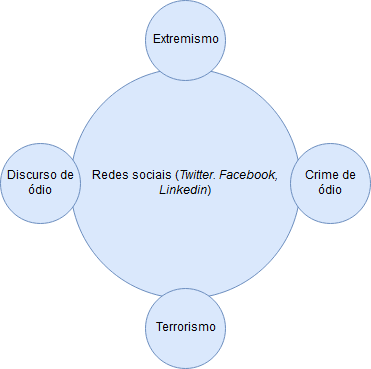
\includegraphics[scale=0.70]{imagens/atividadesdestrutivas.png}
\legend{Fonte: \cite{Chetty2018}}
\label{fig:atividadesdestrutivas}
\end{figure}

O terrorismo é um fenômeno global que resulta na morte de pessoas inocentes e na destruição de propriedades públicas em uma escala gigantesca. Os dois objetivos principais do terrorismo são criar o terror propriamente dito para as vítimas e atrair a atenção das mídias e dos poderes mundiais. O terrorismo é uma ameaça que não distingue raça, religião, nacionalidade e nem gênero, atingindo toda a humanidade \cite{Chetty2018}.

O extremismo é uma ideologia político-religiosa se opondo às normas da sociedade sendo muito semelhante ao terrorismo. Para \citeonline{Liebman1983}, o extremismo é "um desejo de ampliar o escopo, o detalhamento e o rigor da lei religiosa, o isolamento social e a rejeição da cultura periférica." \cite{Liebman1983,Chetty2018}. Muitas vezes, tanto o extremismo como o terrorismo levam ao discurso de ódio e ao crime de ódio.

O crime de ódio é todo ataque físico motivado por ódio contra um indivíduo, propriedade ou comunidade sendo essas violências motivadas pela oposição a religião, ao gênero, a raça, a etnia e a nação. O crime de ódio geralmente é um tipo de crime extremista e punível pela lei constitucional de cada país diferentemente do discurso de ódio que é um tipo de ataque verbal e de difícil punição \cite{Chetty2018}.

O discurso de ódio tem como alvo grupos de minorias sendo mais destrutivo e perigoso quando atinge um símbolo tradicional, evento ou atividade. Os discursos que falam da nação, raça, etnia, religião, orientação sexual, gênero e deficiência geram maiores danos ao indivíduo do que características individuais da vítima. Sendo assim \citeonline{Chetty2018} definem o discurso de ódio como "qualquer fala que ataca um indivíduo ou um grupo com a intenção de ferir ou desrespeitar com base na identidade de uma pessoa" \cite{Chetty2018}.

Um discurso de ódio que não incite a violência e a discriminação também é considerado como prejudicial e, portanto, continua sendo considerado como discurso de ódio já que propósito e ação do autor podem descrever o ato de ódio indireto. A Figura \ref{fig:tiposdediscursodeodio} apresenta os principais temas abordados nos discursos de ódio atualmente dentro das redes sociais.

\begin{figure}[!h]
\centering 
\caption{Tipos de discurso de ódio}
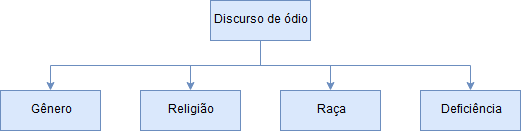
\includegraphics[scale=0.70]{imagens/tiposdediscursodeodio.png}
\legend{Fonte: O Autor}
\label{fig:tiposdediscursodeodio}
\end{figure}

\subsection{Discurso de Ódio de Gênero}
São ataques realizados com base no sexo ou gênero da vítima. As vitimas desse tipo de discurso geralmente são mulheres e garotas, são discursos que denigrem a identidade feminina e que podem acarretar em problemas sociais graves. Esses discursos de ódio também são conhecidos como discurso de ódio sexista e crescem a cada dia devido a facilidade de acesso à \textit{internet} tornando essas agressões mais simples \cite{Chetty2018}.

Tanto as mulheres como os muçulmanos são os maiores alvos de discurso de ódio. Como consequência dessa violência e assédio muitas mulheres se inserem em organizações terroristas, onde as mulheres mais jovens são empregadas como domésticas, prestando serviços domésticos e também serviços sexuais aos integrantes dessas organizações. \cite{Edwards2016}. Muitas mulheres se casam com os homens terroristas como forma de retribuição aos serviços prestados. Já outras são abusadas sexualmente por vários integrantes gerando outro crime grave de abuso sexual que não será abordado nesse trabalho \cite{Edwards2016}.

A alta no número de usuários das redes sociais enfraqueceu as leis desenvolvidas para governar e controlar a \textit{internet}. Muitas ativistas feministas também são alvos de discurso de ódio em meios \textit{online} conforme estudo de 
\citeonline{Hardaker2016}. Como solução para esses assédios que incluem ameaças de estupro cotra as ativistas muitas abordagens são adaptadas conforme situação para rumar a uma igualdade jurídica \cite{Levy2017}. 

\subsection{Discurso de Ódio de Religião}
Esse tipo de ataque é contra religiões como o islamismo, o hindu, e o cristianismo. Como a religião é coletiva, os discursos de ódio são muito mais prejudiciais do que para um único indivíduo. Os muçulmanos são demonizados com atitudes negativas, estereótipos, discriminação e ataques físicos \cite{Chetty2018}. Uma das razões para esses atos de violência é a inclusão dos muçulmanos em grupos extremistas externos e homogêneos envolvidos em conflitos e violência \cite{Trnberg2016}.  

A roupa que um indivíduo veste pode fornecer algumas informações incompletas sobre o mesmo. Muitos indivíduos atribuem o \textit{hijab}\footnote{\textit{Hijab} é o conjunto de vestimentas preconizado pela doutrina islâmica. No Islã, o \textit{hijab} é o vestuário que permite a privacidade, a modéstia e a moralidade, ou ainda "o véu que separa o homem de Deus". \cite{9780742562967}} aos mesmos grupos extremistas terroristas sem ter o conhecimento prévio sobre a religião. Houve um aumento considerável na disseminação de discursos de ódio de religião contra muçulmanos após ataques terroristas em Paris, Tunísia e Woolwich. Além dos ataques verbais, mesquitas foram vandalizadas, \textit{hijabs} foram queimados, torturas físicas foram executadas em homens e propriedades muçulmanas foram destruídas \cite{Awan2016,Chetty2018}.

No meio digital os assédios acontecem por meio de intimação, incitação e ameaças que indicam as violência citadas no parágrafo anterior. Por causa desse comportamento, muitos muçulmanos, por medo de receberem violência gratuita, se retiraram das redes sociais como forma de proteção \cite{Chetty2018}.

\subsection{Discurso de Ódio de Raça}
Esse tipo de violência diz respeito a qualquer expressão em relação à aparência de uma pessoa ou de um grupo. A frequência bem como o impacto dos discursos de ódio racistas depende da intenção e da percepção do governo da nação em que o evento ocorre, variando de liderança para liderança. Segundo \citeonline{tatum2001defining}, "o racismo é um sistema que envolve mensagens culturais e políticas e práticas institucionais, bem como as crenças e ações dos indivíduos" \cite{tatum2001defining}.

As redes sociais tem papel significativo na disseminação do racismo e hoje são a fonte para a compreensão do mesmo. Elas fornecem um contexto para aprender, desafiar e abordar as questões relacionadas ao racismo.  \cite{Chetty2018}. Um exemplo claro foi apresentado por \citeonline{Chaudhry2016} em seu estudo que mostrou que após a morte de um jovem negro  chamado Mike Brown, morto por um tiro dado por Darren Wilson, a maioria dos \textit{tweets} que falavam sobre o tema eram de pessoas negras \cite{Chaudhry2016}.

\subsection{Discurso de Ódio de Deficiência}

Esse tipo de violência é realizado quando condições físicas e mentais de uma pessoa, ou grupo são ridicularizadas. A deficiência é considerada uma categoria social, como é o caso do gênero e da raça de um indivíduo. Incapacidade é qualquer problema de saúde de um indivíduo que o limite na realização das atividades de sua vida. As pessoas sem deficiência são consideradas temporariamente sãs \cite{doi:10.1086/ahr/108.3.763}. Por causa da sua fragilidade, o discurso de ódio de deficiência é mais comum do que para as pessoas saudáveis \cite{Chetty2018}. Mulheres com deficiência intelectual são mais vulneráveis à violência em casa \cite{McCarthy2017}. 

Mesmo sendo grande o número de deficientes vítimas de discurso de ódio, os mecanismos de defesa para esse grupo de indivíduos são menores e muitas vezes inexistentes. Para manter a dignidade dessas pessoas, os governos locais são obrigados a ter sistemas adequados de informação e punição dos crimes \cite{Macdonald2017}.

O crime de mate é um ato contra pessoas com deficiência que é realizado pelos amigos, parentes, ou familiares da própria vítima e é mais semelhante à violência doméstica e necessita ser punido como qualquer outro tipo de discurso de ódio \cite{Chetty2018}. 

\section{Trabalhos Relacionados}
A quantidade de trabalhos que tratam da Análise de Sentimentos é cada vez maior, já que têm o objetivo de estimar o sentimento envolvido em grandes quantidades de dados. O objetivo dessa sessão é apresentar os principais estudos já desenvolvidos, que possuam algum ponto em comum com os objetivos aqui apresentados. Sendo assim, ao final será possível verificar as diferentes implementações e resultados encontrados para auxiliar no desenvolvimento do trabalho.

\subsection{Análise dos sentimentos expressos na rede social \textit{Twitter} em relação aos filmes indicados ao \textit{Oscar} 2017}

O trabalho realizado por \citeonline{Correa2017} abordou os conceitos da Análise de Sentimentos aplicados à rede social \textit{Twitter}, analisando as reações dos usuários em relação aos filmes indicados à categoria de "Melhor Filme" do \textit{Oscar 2017} já que as redes sociais são espaços que possibilitam a divulgação de filmes e também são utilizadas como fonte de opiniões. 

Após realizar a etapa de coleta de informação, \citeonline{Correa2017} gerou uma base de dados rotulada manualmente, distribuída conforme a Tabela \ref{tab:sumarizacaocorrea}. Com a base rotulada já obtida, o autor realizou etapas de pré-processamento para diminuir ruídos de dados removendo \textit{links}, caracteres não alfabéticos e pontuação, removendo repetição de letras e etc.

\begin{table}[h!]
  \begin{center}
    \caption{Sumarização dos dados contidos em base rotulada}
    \label{tab:sumarizacaocorrea}
    
    \begin{tabular}{cc} % <-- Alignments: 1st column left, 2nd middle and 3rd right, with vertical lines in between
      \textbf{Sentimento} & \textbf{Quantidade de \textit{tweets}}\\
      \hline
       positivo&1.444\\
       negativo&1.362\\
       neutro&429\\
      \hline
      Total&3.235
    \end{tabular}
  \end{center}
  \legend{Fonte: \cite{Correa2017}}
\end{table}


Diferentes abordagens de classificação foram apresentadas pelo autor. Desde algoritmos de aprendizado supervisionado (\textit{Naive Bayes}) até o aprendizado por supervisão à distância (utilizando a ferramenta \textit{Sentiment140}\footnote{\url{http://www.sentiment140.com/}}). Para o desenvolvimento foi utilizado o algoritmo \textit{Naive Bayes} por ser o mais utilizado em casos de bases rotuladas, aplicando a base rotulada no \textit{software Weka} \cite{Correa2017}. 

O autor concluiu que o nível de acurácia apresentada pela classificação de base de dados rotulada apresentada pelo algoritmo \textit{Naive Bayes} multinomial foi de $75\%$, sendo bastante indicado para tarefas semelhantes. Também foi possível concluir que parte considerável dos usuários do \textit{Twitter} prefere usar a ferramenta para publicar comentários positivos sobre os filmes, já que os mesmos permaneceram ativos e animados na rede social durante a semana em que foram divulgados os indicados ao \textit{Oscar 2017} \cite{Correa2017}.

Para os próximos trabalhos, dentre as demais sugestões do autor, está o estudo dos perfis de usuários considerando apenas os \textit{tweets} publicados pelos usuários do perfil desejado. Também é sugerido realizar estudos utilizando uma base de dados composta por \textit{tweets} publicados após o \textit{Oscar} gerando tabela comparativa \cite{Correa2017}.

\subsection{Detecção de Tweets contra Afro-americanos}

No trabalho proposto por \citeonline{kwok2013locate} tem-se um estudo sobre o discurso de ódio contra os afro-americanos usuários do \textit{Twitter}. Esses discursos de ódio são especialmente penais dentro da rede social em questão, embora esse efeito não seja percebido em meio aos dados gerados diariamente dentro da plataforma.

Para realizar o desenvolvimento, os autores coletaram uma centena de \textit{tweets} que continham palavras-chave geralmente encontrados em discursos de ódio, e pediram a três estudantes de diferentes etnias (de mesma idade e sexo) para avaliarem cada um dos textos com uma nota de 1 (um) à 5 (cinco) conforme o grau de ofensa que o estudante julgasse ter o texto. O resultado foi de $33\%$ de concordância entre os estudantes mostrando que utilizar a abordagem estatística \textit{Fleiss' Kappa} seria ainda de menor precisão se realizado por uma máquina \cite{kwok2013locate}.

Para realizar a classificação dos dados previamente rotulados entre dados racistas e dados não racistas, foi utilizado o algoritmo de \textit{Naive Bayes} já que o mesmo, segundo os autores, funciona tão bem quanto os algoritmos mais sofisticados.

Os \textit{tweets} racistas foram coletados a partir de contas que foram auto-classificadas como racistas ou consideradas racistas por meio de notícias. Os autores chegaram em uma base rotulada de $24.582$ \textit{tweets} pré-processados, onde as URLs foram removidas, as palavras foram padronizadas em letras minúsculas, palavras irrelevantes foram removidas e a grafia de palavras de insulto foram substituídas pelo seu equivalente soletrado corretamente \cite{kwok2013locate}.

Após a classificação, os autores concluíram que termos como \textit{niggers} e \textit{nig-er} são padrão para insultar negros, enquanto as palavras \textit{niggas} e \textit{nigga} se limitam à fala coloquial geralmente utilizada pela comunidade negra. Esses termos não têm conotação racial porém o uso é restrito a negros e a pessoas aprovadas pela comunidade negra \cite{kwok2013locate}.

Por fim, \citeonline{kwok2013locate} concluem que a base de dados apurada por eles não foi suficiente para classificar com total precisão os \textit{tweets} de origem racista e afirmam que esse desafio deve ser a motivação para que novas pesquisas ocorram e que novos refinamentos ocorram nos métodos de classificação apresentados pelos seu trabalho.

\subsection{Comentários Ofensivos na Internet Brasileira}

Em seu trabalho, \citeonline{Pelle2017} constataram que as redes sociais são ferramentas que trazem a liberdade para o usuário poder apresentar suas ideias e compartilhar informações. Entretanto, percebem que essa mesma ferramenta está cheia de usuários que promovem o discurso de ódio. A análise desses eventos é inviável de forma manual uma vez que a cada dia muito mais textos são gerados.

É nesse contexto que \citeonline{Pelle2017} verificam a necessidade de uma ferramenta que realize essa análise de forma automática e propõem o desenvolvimento da mesma para a língua portuguesa, já que atualmente existem poucas abordagens específicas para o idioma. Para realizar o experimento, os autores desenvolveram uma base de dados rotulada especifica para a língua portuguesa, buscando por discursos de ódio dentro do site \textit{g1.globo.com}\footnote{ Classificado como o site mais acessado no Brasil em 2017, pelo site  \url{http://www.alexa.com/topsites/countries/BR}} (\url{https://g1.globo.com}) e classificando os comentários entre discursos negativos e discursos positivos. Com essa coleta, constatou-se que $90\%$ das notícias publicadas no site tinham ao menos um discurso de ódio em seus comentários e após uma análise preliminar foi descoberto que as categorias com a maior parte de discursos de ódio foram \textit{política} e \textit{esportes}.

Com uma base composta por $10.336$ comentários oriundos de $115$ notícias, os autores escolheram $1.250$ comentários de forma aleatória para serem rotuladas por três pessoas que julgavam os texto e, em caso de detectarem um texto ofensivo, os juízes deveriam ainda categorizar a ofensa como racismo, sexismo, homofobia, xenofobia, intolerância religiosa ou xingamento \cite{Pelle2017}. 

Para realizar a classificação da base rotulada, \citeonline{Pelle2017} utilizaram o \textit{software} \textit{Weka} e testaram os algoritmos \textit{Naive Bayes} e \textit{SVM} (sendo chamado de \textit{SMO} na implementação do \textit{Weka}) por serem amplamente usados em rotinas de mineração de textos \cite{Pelle2017}. 

Ao final concluiu-se que de fato existem poucas literaturas que abordam o discurso de ódio na \textit{internet} analisando a língua portuguesa e que, para os próximos estudos, é possível realizar um estudo com maior carga de dados rotulados utilizando métodos de \textit{crowdsourcing}, também é visto a possibilidade de mapear o usuário gerador de discursos de ódio para que se saiba o perfil desses usuários \cite{Pelle2017}.

\subsection{Revisão de Ferramenta Implementada}
\label{sec:revisaoferramenta}
Com o crescimento das pesquisas no campo da mineração de texto e com as variadas aplicações encontradas para a Análise de Sentimentos, cada vez mais ferramentas são desenvolvidas com os mais variados propósitos de pesquisa, e também para aplicações comerciais. A ferramenta base para o trabalho aqui desenvolvido é resultado de uma pesquisa realizada por \citeonline{tccfilipe} que resultou em um \textit{software} \textit{web crawler}\footnote{ \textit{Softwares} que criam conexão com determinado \textit{site} e extraem informações desejadas por meio de APIs geralmente disponibilizadas pelo meio eletrônico \cite{Kumar2018}.} que realiza a Análise de Sentimentos em uma interface relativamente simples para usuários que não têm experiência em programação.

É possível verificar na Figura \ref{fig:fluxotccfilipe} o fluxo de funcionalidades da ferramenta implementada onde, inicialmente, o usuário entra com uma URL de busca e a quantidade de postagens a ser analisada (Figura \ref{fig:menutccfilipe}) e após ocorre a classificação. Por fim ocorre a apresentação das informações em forma de nuvem de palavras (Figura \ref{fig:nuvemtccfilipe}), gráficos (Figura \ref{fig:graficotccfilipe}), e ainda, em relatórios gerados em PDF (Figura \ref{fig:exportadotccfilipe}). A coleta de dados ocorreu com a API apresentada na Sub-sessão \ref{subsec:coletadados} chamada \textit{Facebook Graph API}, a partir dela o \textit{software} faz buscas na rede social \textit{Facebook} e coleta postagens conforme parametrizado.

\begin{figure}[!h]
\centering 
\caption{Fluxograma de funcionalidades do \textit{software} revisado}
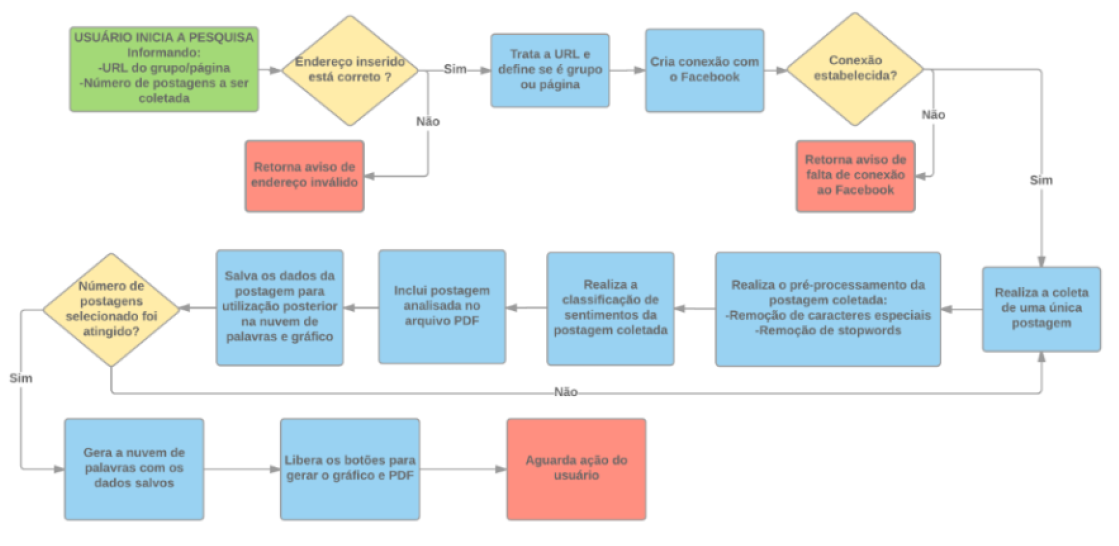
\includegraphics[scale=0.44]{imagens/fluxofilipe.png}
\legend{Fonte: \cite{tccfilipe}}
\label{fig:fluxotccfilipe}
\end{figure}

\begin{figure}[!h]
\centering 
\caption{Menu de busca do \textit{software} revisado}
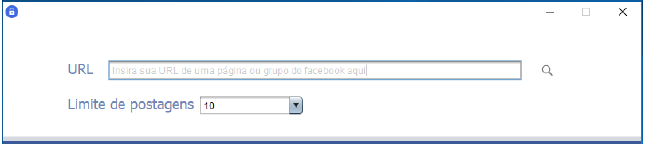
\includegraphics[scale=0.6]{imagens/menudebuscafilipe.png}
\legend{Fonte: \cite{tccfilipe}}
\label{fig:menutccfilipe}
\end{figure}

\begin{figure}[!h]
\centering 
\caption{Nuvem de palavras do \textit{software} revisado}
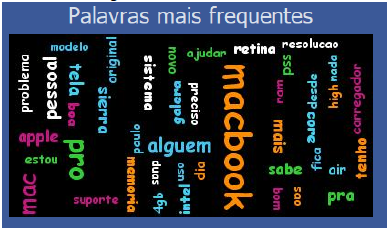
\includegraphics[scale=0.62]{imagens/nuvemdepalavras.png}
\legend{Fonte: \cite{tccfilipe}}
\label{fig:nuvemtccfilipe}
\end{figure}

\begin{figure}[!h]
\centering 
\caption{Gráfico de sentimentos do \textit{software} revisado}
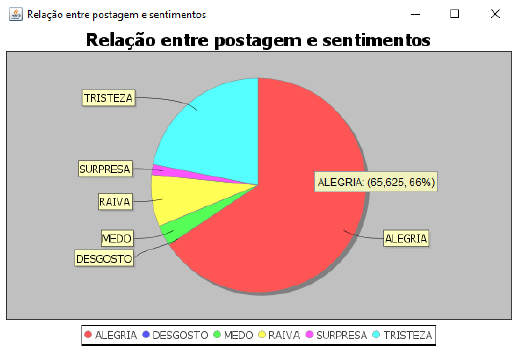
\includegraphics[scale=0.8]{imagens/graficodesentimentosfilipe.png}
\legend{Fonte: \cite{tccfilipe}}
\label{fig:graficotccfilipe}
\end{figure}

\begin{figure}[!h]
\centering 
\caption{Resultado exportado do \textit{software} revisado}
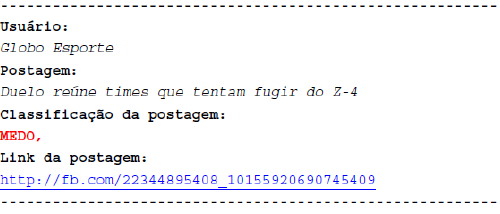
\includegraphics[scale=0.60]{imagens/exportadofilipe.png}
\legend{Fonte: \cite{tccfilipe}}
\label{fig:exportadotccfilipe}
\end{figure}

\newpage
Para atingir o propósito de sua pesquisa, \citeonline{tccfilipe} realizou o estudo de léxicos de emoções contidos na base de dados chamada \textit{WordNet}\footnote{\url{https://wordnet.princeton.edu}} categorizados em seis grupos distintos que foram: alegria, desgosto, medo, raiva, surpresa e tristeza. Na Tabela \ref{tab:categoriaemo} estão alguns exemplos de palavras separadas pelas respectivas categorias de emoção selecionado pelo autor. Além da Análise de Sentimentos também foi implementada busca por palavras frequentemente encontradas em ataques de \textit{phishing},  e também palavras de linguagem imprópria, visto que as redes sociais não mantém um filtro de conteúdo levando em consideração a idade do usuário.

\begin{table}[h!]
  \begin{center}
    \caption{Categorias de emoções}
    \label{tab:categoriaemo}
    \begin{tabular}{ll} % <-- Alignments: 1st column left, 2nd middle and 3rd right, with vertical lines in between
      \textbf{Categoria} & \textbf{Palavras}\\
      \hline
      Alegria&animação, ânimo, comédia\\
      Desgosto&maldoso, chatear, abominável\\
      Medo&desespero, escuridão, friamente\\
      Raiva&assassinar, bravejar, detestar\\
      Surpresa&chocante, espanto, impressionado\\
      Tristeza&cabisbaixo, chorão, culpa\\
      \hline
    \end{tabular}
  \end{center}
  \legend{Fonte: \cite{tccfilipe}}
\end{table}
Após definir os grupos de coleta, os dados de coleta para a Análise de Sentimentos e realizar a classificação dos dados utilizando método de classificação baseado em léxicos, o autor realizou a análise dos resultados para constatar o quão precisa foi a classificação realizada pela ferramenta. \citeonline{tccfilipe} coletou amostras de diferentes tamanhos em todos os grupos analisados totalizando 50 (cinquenta), 100 (cem) e 500 (quinhentos) postagens para, após, serem também analisadas manualmente e assim comparar os resultados. Dentre os grupos estudados estão a página do \textit{Outback Brasil} e o grupo da Previdência Social, alguns ajustes de léxicos foram necessários para que as classificações ocorressem com maior assertividade nos casos de alegria e tristeza. No final foi realizada a comparação entre as classificações e exatificadas as suas respectivas taxas de acerto, a Tabela \ref{tab:taxaacerto} apresenta os resultados obtidos, com eles foi possível verificar que quatro dos sentimentos tiveram taxa de acerto superiores a oitenta por cento. Com o cálculo do desvio padrão foi possível constatar que nos sentimentos com menor classificação refletiam uma grande dispersão em torno da media populacional, resultado de expressões ambíguas e de duplo sentido.

\begin{table}[h!]
  \begin{center}
    \caption{Taxa média de acerto na classificação de postagens analisadas}
    \label{tab:taxaacerto}
    \begin{tabular}{lllllll} % <-- Alignments: 1st column left, 2nd middle and 3rd right, with vertical lines in between
      \textbf{Classificação} & \textbf{Alegria} & \textbf{Medo} & \textbf{Tristeza} & \textbf{Desgosto} & \textbf{Raiva} & \textbf{Surpresa}\\
      \hline
      Taxa de Acerto&52,82\%&90,77\%&81,55\%&88,89\%&91,01\%&75,83\%\\
      Desvio Padrão($\sigma$)&16,06&2,62&5,20&4,61&4,23&9,97\\
      \hline
    \end{tabular}
  \end{center}
  \legend{Fonte: \cite{tccfilipe}}
\end{table}

Ao final dos estudos foi concluído que a ferramenta desenvolvida trouxe resultados satisfatórios tanto pelos resultados obtidos como pela facilidade que a ferramenta desenvolvida trás para os usuários comuns. Ainda, foram apontadas melhorias para os estudos futuros entre elas o desenvolvimento de uma plataforma \textit{web}, aprimoramento nos testes de resultados da Análise de Sentimentos e também novas abordagens na etapa de classificação dos dados. 
% falar aqui sobre os resultados encontrados pelo filipe

\section{Considerações Finais}
A Análise de Sentimentos (SA), é a classificação de um dado textual baseado no seu teor sentimental, de opinião, avaliação de atitudes e é amplamente utilizada para a avaliação de determinadas entidades como eventos, produtos, problemas sociais, entre outros. Essa técnica é cada vez mais necessária, uma vez que atualmente se torna inviável a análise manual realizada por especialistas humanos, pois a cada dia, milhões de novos textos são gerados na \textit{internet} \cite{BAHRI2018669}.

Com o avanço tecnológico, a forma de o seres-humanos compartilharem informações também mudou e hoje as redes sociais vão além de plataformas de comunicação e troca de informações, elas conseguem até impactar no crescimento econômico de uma nação. \textit{Facebook}, \textit{Twitter}, \textit{Youtube} são exemplos de redes sociais que estão entre as mais utilizadas atualmente, seja para troca de fotos e vídeos, seja para o compartilhamento livre de opiniões e cultura. Porém, essa liberdade de expressão também trouxe um fenômeno negativo para a população, os discursos de ódio praticados pelos \textit{haters} de \textit{internet} que tem o mesmo poder destrutivo que as agressões físicas e verbais \textit{offline}. 

Foi visto, em um estudo realizado por \citeonline{Chetty2018}, que os discursos de ódio são geralmente categorizados entre quatro principais temas que são: gênero, religião, raça e deficiência, sendo puníveis, dependendo do governo atuante de cada nação. No estudo realizado por \citeonline{Chetty2018} também foi possível verificar que os maiores alvos de discurso de ódio são os muçulmanos, enquanto os maiores alvos de violência física são as mulheres com deficiência física, ou deficiência intelectual.

Com os trabalhos relacionados foi possível perceber que a Análise de Sentimentos é uma área amplamente necessária. Nos estudos realizados por \citeonline{Correa2017} foi possível perceber os métodos de classificação mais utilizados e também a importância de uma base de dados rotulada para aprendizado de máquina, no qual o contexto de \textit{Oscar} fomentou a pesquisa para buscar a opinião dos usuários sobre os filmes em destaque. Já no trabalho desenvolvido por \citeonline{kwok2013locate} foi possível perceber a necessidade da Análise de Sentimentos em desafios sociais, mais especificamente o racismo. Em seu trabalho os autores buscaram montar uma Análise de Sentimentos que detectava discursos de ódio específicos para a comunidade negra americana e foi de suma importância para o objetivo do nosso trabalho de buscar discursos de ódio na rede social \textit{Twitter}. Por fim, com os estudos realizados por \citeonline{Pelle2017} foi possível afirmar que, de fato, hoje existem poucas obras disponíveis voltadas para o discurso de ódio na língua portuguesa. Também é difícil encontrar ferramentas e bases de dados para o idioma, o que fomenta o desafio para a comunidade cientifica brasileira.

É com essas conclusões que o trabalho de gerar uma base de léxicos para discursos de ódio específico para a língua portuguesa se mostra ser importante para a comunidade. O desafio se mostra necessário para que se possa detectar discursos de ódio que a cada dia aumentam em nossa sociedade.
\chapter{Desenvolvimento}
\label{cap:Desenvolvimento}
Nesse capítulo serão abordadas todas as etapas, tal como as técnicas utilizadas para atingir o objetivo de compor um dicionário de léxicos da língua portuguesa específico para detecção de discursos de ódio promovido pelos usuários chamados de \textit{haters}. Também será apresentada ferramenta implementada que será utilizada como base para as novas funcionalidades e testes com os novos léxicos utilizados .Ao final, também serão apresentados os resultados esperados com o desenvolvimento, estimando a eficiência e os avanços da pesquisa realizada. 

\section{Geração de \textit{corpus} para Detectar \textit{Haters}}
\label{sec:geracaohater}
Como parte fundamental da pesquisa, será criado um dicionário com as palavras mais utilizadas pelos usuários denominados \textit{haters} que pregam discursos de ódio contra indivíduos nas redes sociais. Para a geração do \textit{corpus} desejado serão necessárias algumas etapas de desenvolvimento como pode ser visto na Figura \ref{fig:fluxodesenvolvimento}. A seguir serão explicadas cada uma das etapas a serem realizadas para a obtenção do novo dicionário.

\begin{figure}[!h]
\centering 
\caption{Fluxo de atividades para obtenção de \textit{corpus} desejado}
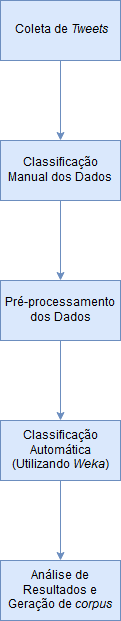
\includegraphics[scale=0.45]{imagens/fluxodesenvolvimento.png}
\legend{Fonte: O Autor}
\label{fig:fluxodesenvolvimento}
\end{figure}

\subsection{Coleta de \textit{Tweets}}
\label{subsec:coletatweets}
A plataforma selecionada para a coleta de dados textuais será o \textit{Twitter}, rede social categorizada como \textit{microblogging} em que os usuários realizam atualizações constantes de conteúdo, sendo esse conteúdo textual, figuras, vídeos, enquetes entre outros. No contexto da rede social, as postagens dos usuários recebem o nome de \textit{tweet} e tem o limite de $280$ caracteres. 

Para realizar a coleta de dados primeiramente é necessário criar uma conta dentro da \textit{Twitter Developer Platform}\footnote{https://developer.twitter.com/} informando alguns tópicos básicos sobre o uso dos dados e a finalidade da ferramenta a ser desenvolvida. Após cadastro, a plataforma disponibilizará os \textit{tokens}\footnote{chaves de autenticação amplamente utilizadas em implementações \textit{OAuth}.Em que não é necessário informar usuário e senha de acesso à ferramenta} que serão necessários para a construção do programa de leitura de \textit{tweets} (Figura \ref{fig:twitterdeveloperplatform}) bem como um painel para controle de acesso aos dados e renovação das \textit{tokens}.

\begin{figure}[!h]
\centering 
\caption{Tela com \textit{tokens} utilizados na \textit{API} do \textit{Twitter}}
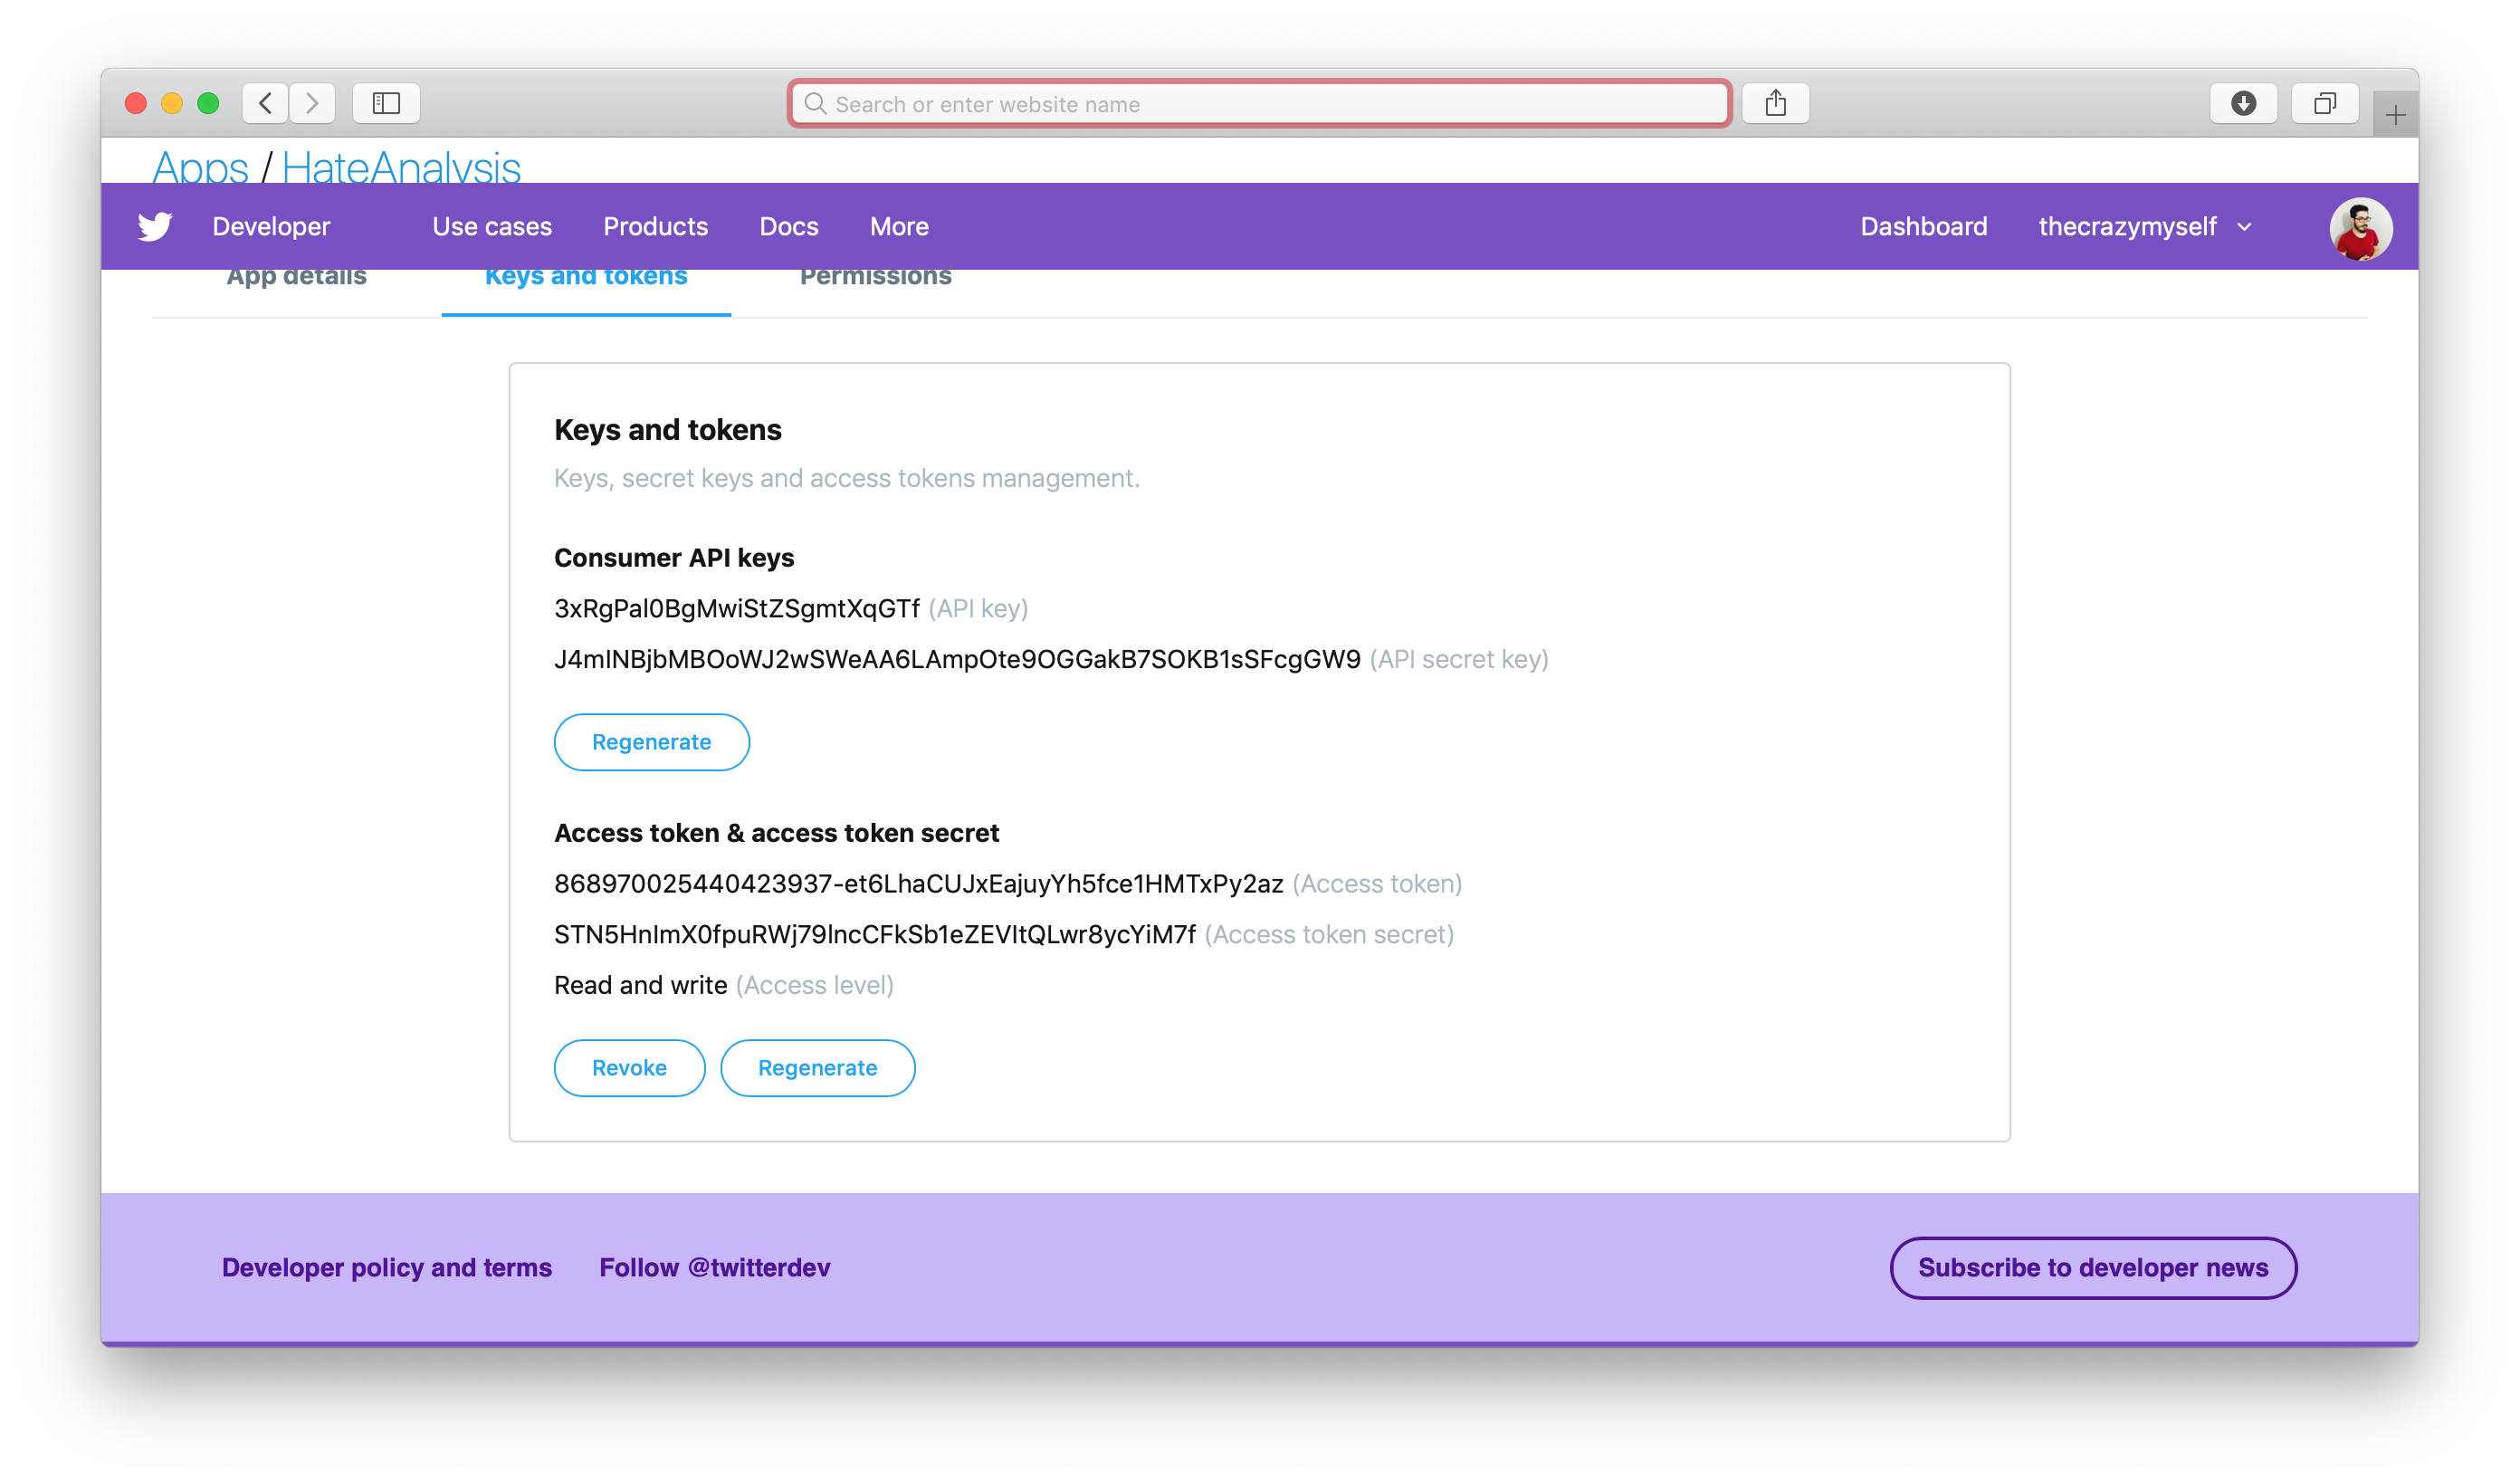
\includegraphics[scale=0.3]{imagens/twitterdeveloperplatform.png}
\legend{Fonte: Twitter Inc.}
\label{fig:twitterdeveloperplatform}
\end{figure}

A linguagem de programação a ser utilizada para a coleta dos dados será a \textit{Java}, linguagem orientada a objetos e multiplataforma mantida pela \textit{Oracle} que é de fácil implementação e bastante utilizada na comunidade \textit{open source} (de código livre) que mantém vários fóruns, \textit{frameworks} e \textit{APIs} constantemente atualizados pela comunidade. A \textit{API} utilizada será a \textit{Twitter4J}\footnote{http://twitter4j.org/en/index.html}, uma biblioteca não-oficial que permite o acesso aos dados do \textit{Twitter} utilizando a linguagem de programação \textit{Java}, a mesma que será utilizada para a coleta de dados, facilitando o aprendizado da ferramenta bem como a manutenção, se necessário. A \textit{Twitter4J} utiliza autenticação \textit{OAuth}, ou seja, fazendo uso dos \textit{tokens} disponibilizados pelo \textit{Twitter Developer Platform} e não necessitando de autenticação com e-mail (ou nome de usuário, e senha) a cada acesso realizado. 

Após a construção do programa de coleta de \textit{tweets}, o próximo passo será encontrar filtros de consulta que irão auxiliar na busca por conteúdos úteis para a geração do \textit{corpus}. O primeiro critério de seleção será a busca por perfis de influenciadores digitais (comumente chamados pela versão inglesa \textit{digital influencers}), que são pessoas que tem grande influência na mídia, tendo vários seguidores e também vários \textit{haters} comentando suas postagens. Nesse primeiro momento os próximos filtros serão manualmente aplicados por um especialista humano que realizará a busca por \textit{tweets} neutros e \textit{tweets} considerados de ódio\footnote{Sendo considerado textos que expressem ideologias onde religião, etnia, deficiências ou gênero são ridicularizados.}. 

A classificação bem como os totais de postagens a serem coletadas pelo especialista podem ser vistos na Tabela \ref{tab:classificacaotweets}.
Após a coleta os dados serão inseridos em arquivos binários e estarão prontos para a próxima etapa prevista para a obtenção do dicionário de léxicos para postagens de \textit{haters} na língua portuguesa.
\begin{table}[h!]
  \begin{center}
    \caption{Classificação dos \textit{tweets} coletados por especialista humano}
    \label{tab:classificacaotweets}
    \begin{tabular}{ll} % <-- Alignments: 1st column left, 2nd middle and 3rd right, with vertical lines in between
    \textbf{Classificação} & \textbf{Quantidade de Tweets}\\
    \hline
    \textit{Tweets} Neutros&500 \textit{Tweets}&
    \textit{Tweets} de Ódio&500 \textit{Tweets}&
    \hline
    Total&1.000 \textit{Tweets}\\
    \end{tabular}
  \end{center}
  \legend{Fonte: O Autor}
\end{table}

\subsection{Classificação Manual dos Dados}
\label{subsec:classmanual}
Nessa etapa, com o auxílio de um especialista humano, os textos apurados na etapa de coleta de \textit{tweets} (Sub-sessão \ref{subsec:coletatweets}) passarão por uma classificação manual como pode ser visto na Figura \ref{fig:classificacaotextos}, afim de gerar uma base de dados para posterior aprendizado de máquina e para comparação estatística de resultados. 
Nessa etapa os textos poderão ser classificados entre duas categorias: \textit{neutro} e \textit{hater}. Onde a primeira categoria compreenderá textos sem nenhum tipo de violência nem extremismo, podendo compreender emoções tanto positivas como negativas. Já a segunda categoria compreenderá textos invasivos, onde a violência verbal seja praticada contra um indivíduo ou um grupo. Dentro desses textos violentos pretende-se também classificar as violências nas subcategorias: racista, religioso, incapacidade e gênero.  

\begin{figure}[!h]
\centering 
\caption{Diagrama de coleta e classificação dos textos}
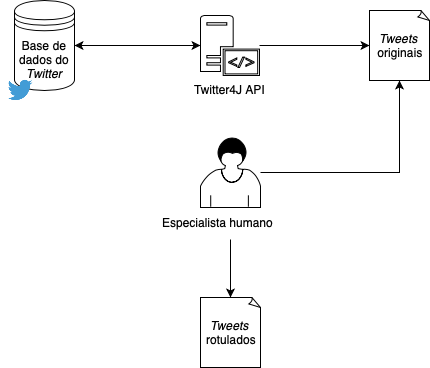
\includegraphics[scale=0.50]{imagens/coletatweets.png}
\legend{Fonte: O Autor}
\label{fig:classificacaotextos}
\end{figure}
\newpage

Com essa etapa pretende-se montar uma base de dados que posteriormente será pré-processada para remoção de ruídos e que irá compor o \textit{dataset} para treinamento dentro do \textit{software weka}. Por isso, é importante que os textos sigam a seguinte formatação: "classificador, racista (true, false), religioso (true, false), incapacidade (true, false), gênero (false),'texto coletado'" como forma de padronização de dados a serem classificados de forma automática como é exemplificado na Figura \ref{fig:arqanalise} onde pode ser verificado um primeiro texto onde um discurso de ódio foi detectado e sub categorizado como ódio a um gênero e já no segundo texto nada foi percebido e portanto o mesmo foi classificado como neutro.

\begin{figure}[!h]
\centering 
\caption{Exemplo de classificação manual }
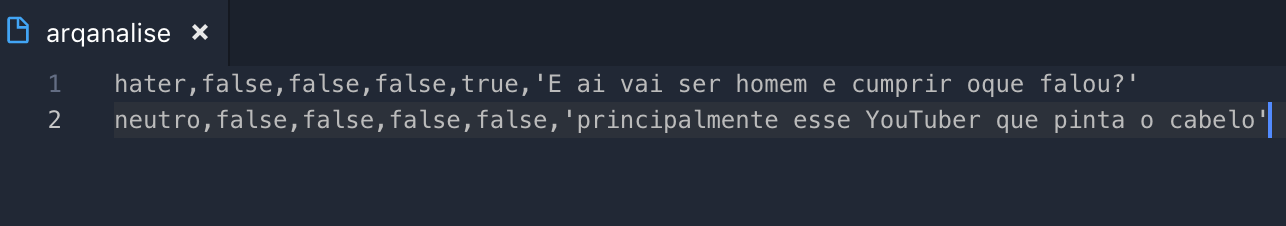
\includegraphics[scale=0.60]{imagens/arqanalise.png}
\legend{Fonte: O Autor}
\label{fig:arqanalise}
\end{figure}

\subsection{Pré-processamento dos \textit{Tweets}}
Assim como visto na Sub-sessão \ref{subsec:preproc}, a etapa de pré-processamento é necessária para a remoção de informações desnecessárias, realizando uma padronização das informações contidas nos textos coletados realizando uma otimização considerável no conteúdo a ser avaliado no processo de classificação automática. 

Para a composição do \textit{dataset} serão realizadas as técnicas de: remoção de conteúdo numérico, remoção de \textit{URL}, remoção de conteúdo numérico, substituição de pontuações repetidas, todas as palavras serão transformadas para letras maiúsculas, remoção de palavras \textit{stopwords} e substituição de palavras alongadas. 

Ao realizar as técnicas citadas anteriormente, será gerado um \textit{dataset} otimizado. O mesmo será utilizado na etapa de classificação e treinamento de máquina para a geração do \textit{corpus} objetivo do trabalho. Posteriormente a mesma rotina de pré-classificação será incorporada em ferramenta desenvolvida citada na Sessão \ref{sec:revisaoferramenta}.

\subsection{Classificação Automática Utilizando o \textit{Weka} e Geração de \textit{corpus}}

Tendo realizado as etapas anteriores de coleta de \textit{tweets}, de classificação manual e de pré-processamento, o próximo passo será a aplicação de algoritmos de \textit{machine learning} para a classificação automática dos dados apurados nas etapas anteriores. A ferramenta utilizada nessa etapa será o \textit{software} chamado \textit{Weka} \footnote{https://www.cs.waikato.ac.nz/ml/weka/}(Figura \ref{fig:telaincialweka}) que é uma coleção de algoritmos de \textit{machine learning} utilizados para tarefas de mineração de dados, contendo ferramentas para preparação, classificação, clusterização, entre outros.  Além de ter ferramentas de visualização de resultados. O \textit{Weka} é um \textit{software} \textit{open source} sob a \textit{GNU General Public License}\footnote{https://www.gnu.org/licenses/licenses.html\#GPL} \cite{weka_2018}.

\begin{figure}[!h]
\centering 
\caption{Tela inicial da ferramenta \textit{Weka}}
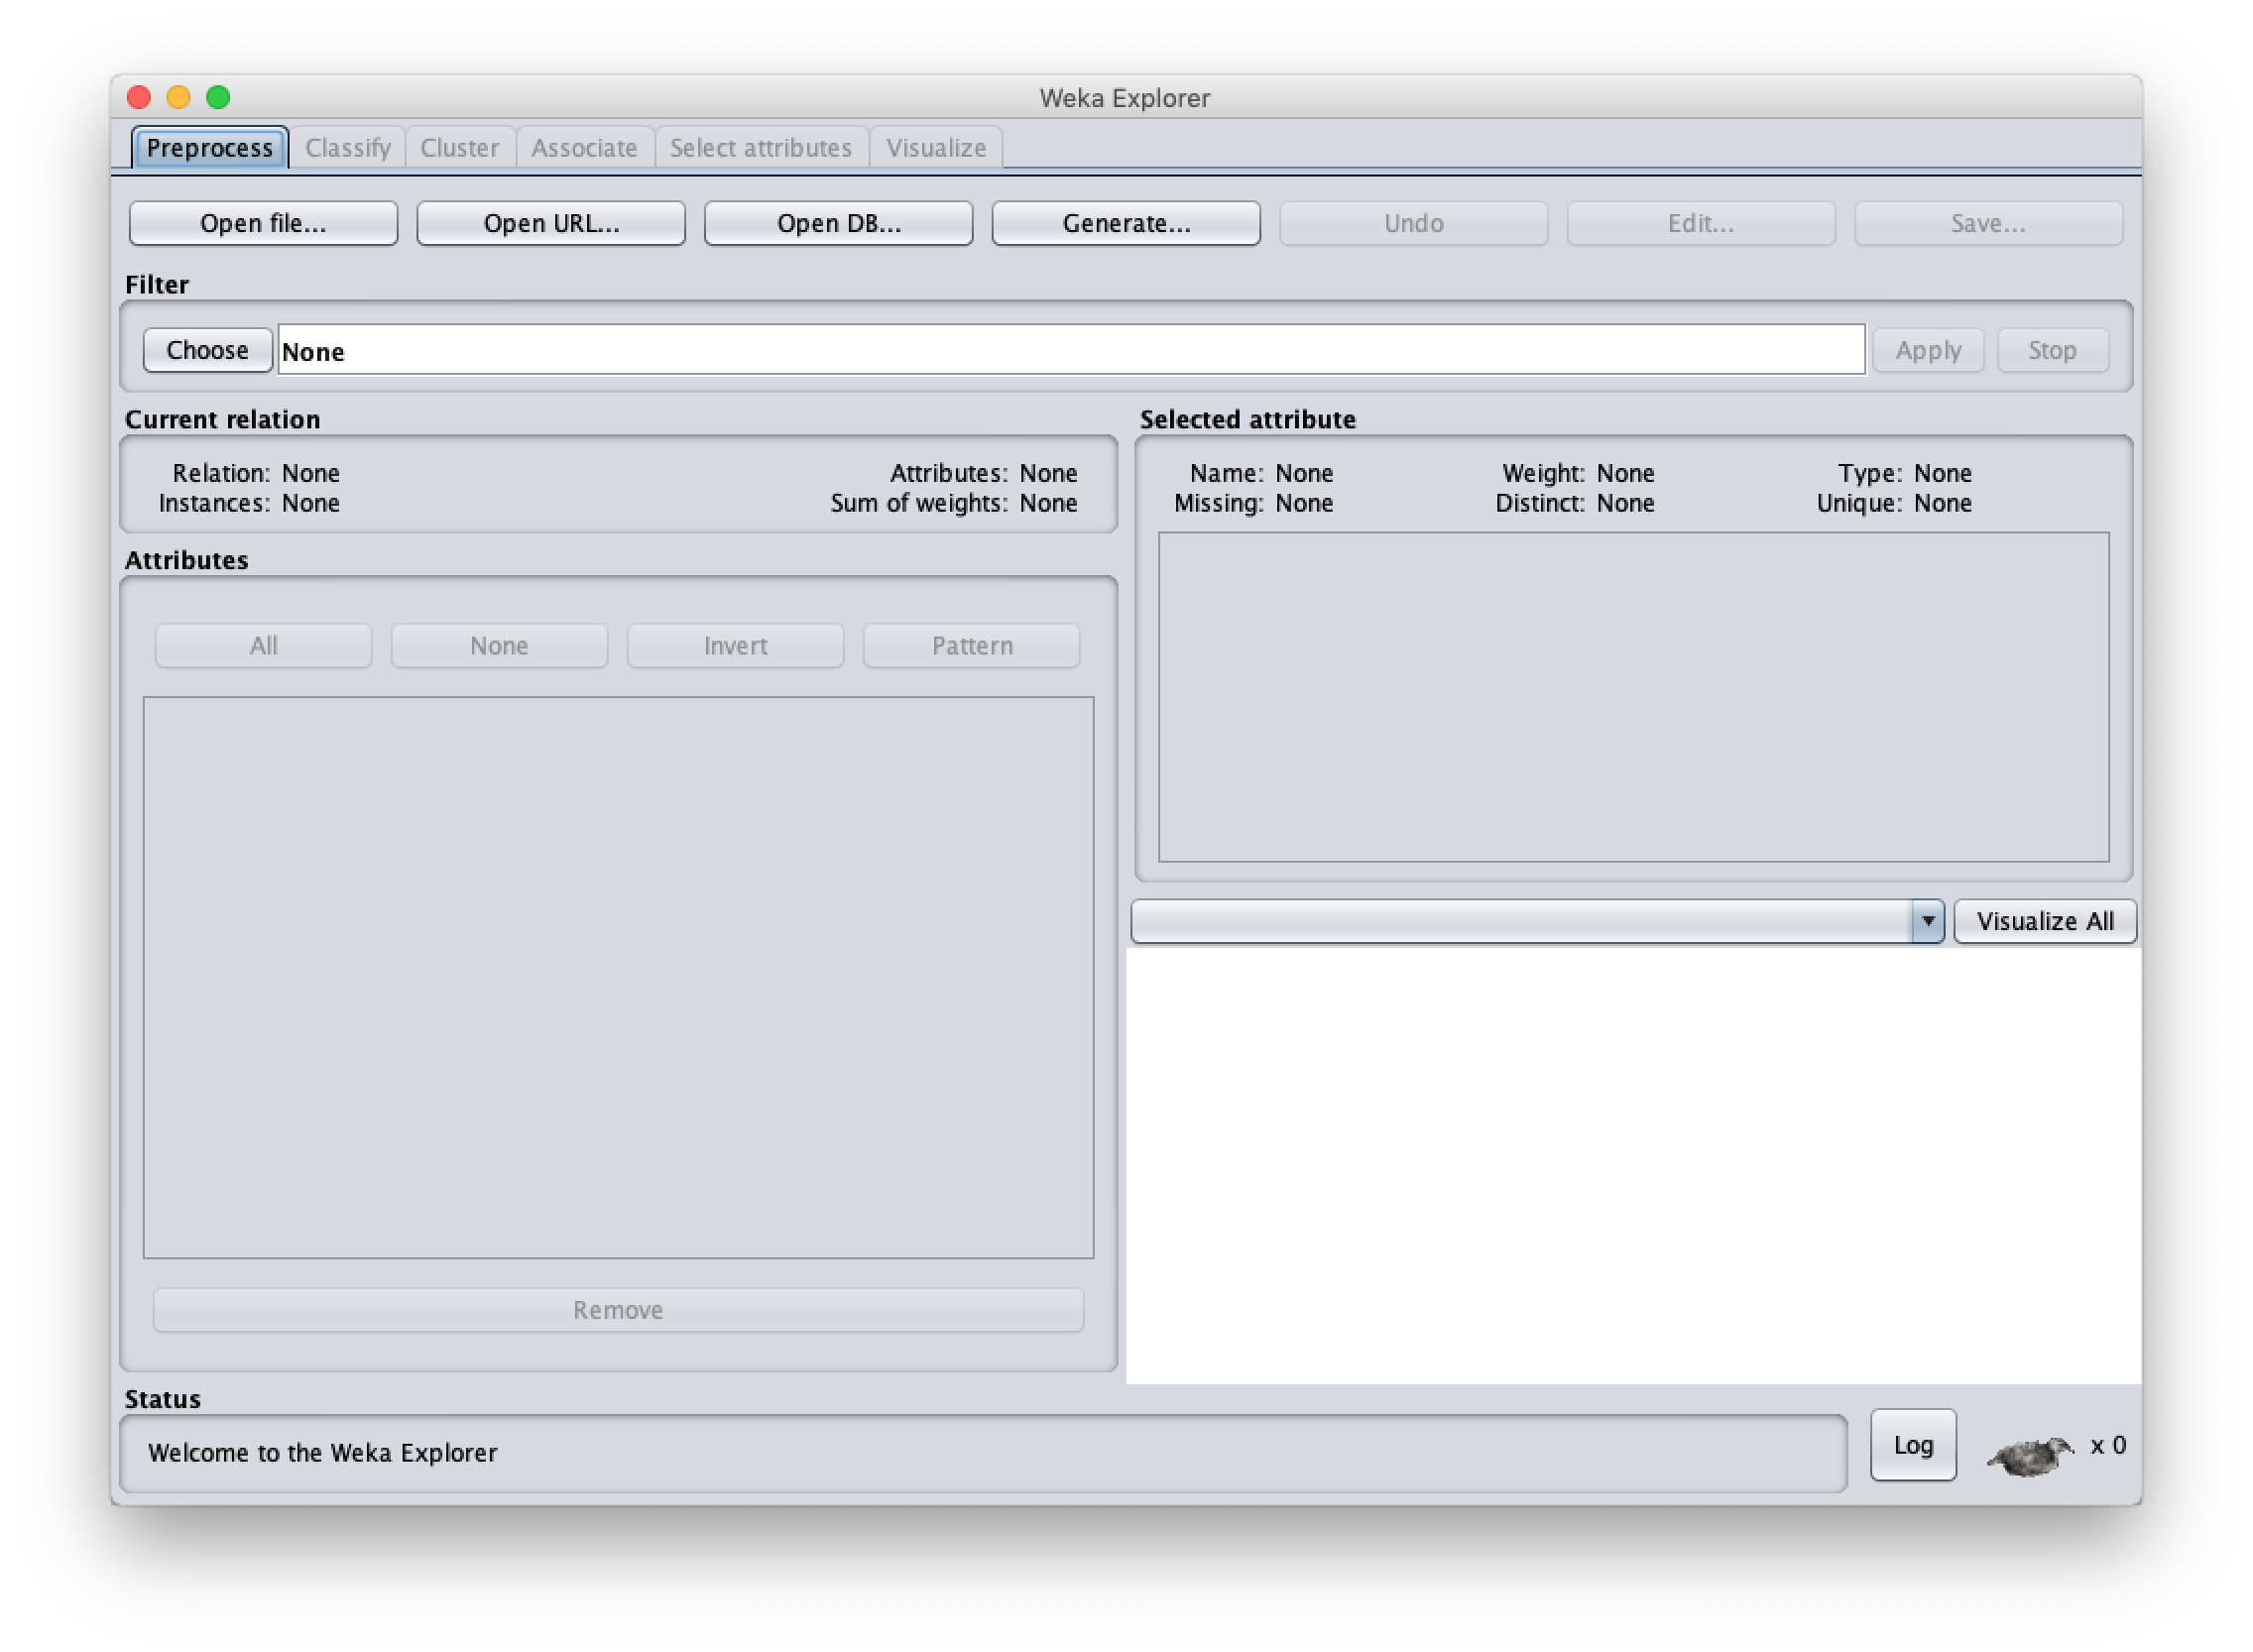
\includegraphics[scale=0.33]{imagens/wekatelainicial.png}
\legend{Fonte: O Autor}
\label{fig:telaincialweka}
\end{figure}

Essa etapa pretende executar três algoritmos de classificação automática de textos para, a partir de seus resultados, gerar o \textit{corpus} com os léxicos mais utilizados nos discursos de ódio. Um esquema com os passos principais pode ser visto na Figura \ref{fig:wekaclassificacao}. Os três algoritmos a serem utilizados nessa etapa são: \textit{Naive Bayes} (NB), \textit{Bayse net} (BN) e \textit{Support Vector Machine} (SVM) \cite{Muralidharan2012,N18-1095}. 

\begin{figure}[!h]
\centering 
\caption{Diagrama da etapa de classificação com o \textit{software} \textit{weka}}
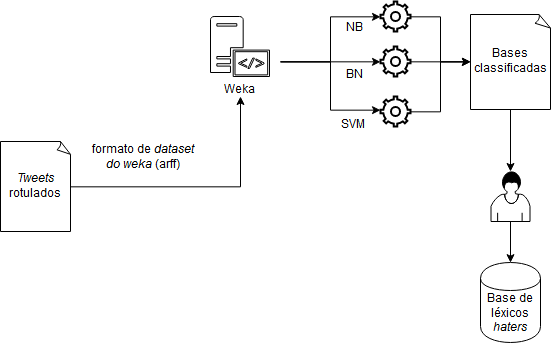
\includegraphics[scale=0.50]{imagens/wekaclassificacao.png}
\legend{Fonte: O Autor}
\label{fig:wekaclassificacao}
\end{figure}

\section{Revisão de Ferramenta Implementada}
\label{sec:revisaoferramenta}
Com o crescimento das pesquisas no campo da mineração de texto e com as variadas aplicações encontradas para a análise de sentimentos, cada vez mais ferramentas são desenvolvidas com os mais variados propósitos de pesquisa e também para aplicações comerciais. A ferramenta base para o trabalho aqui desenvolvido é resultado de uma pesquisa realizada por \citeonline{tccfilipe} que resultou em um software \textit{web crawler}\footnote{ \textit{Softwares} que criam conexão com determinado \textit{site} e extraem informações desejadas por meio de APIs geralmente disponibilizadas pelo meio eletrônico.} que realiza a análise de sentimentos em uma interface relativamente simples para usuários que não têm experiência em programação.

É possível verificar na Figura \ref{fig:fluxotccfilipe} o fluxo de funcionalidades da ferramenta implementada onde, inicialmente, o usuário entra com uma URL de busca e a quantidade de postagens a ser analisada (Figura \ref{fig:menutccfilipe}) e após ocorre a classificação e por fim ocorre a apresentação das informações em forma de nuvem de palavras (Figura \ref{fig:nuvemtccfilipe}), gráficos (Figura \ref{fig:graficotccfilipe}), e ainda, em relatórios gerados em PDF (Figura \ref{fig:exportadotccfilipe}). A coleta de dados ocorreu com a API apresentada na sub-sessão \ref{subsec:coletadados} chamada \textit{Facebook Graph API}, a partir dela o \textit{software} faz buscas na rede social \textit{Facebook} e coleta postagens conforme parametrizado.

\newpage

\begin{figure}[!h]
\centering 
\caption{Fluxograma de funcionalidades do \textit{software} revisado}
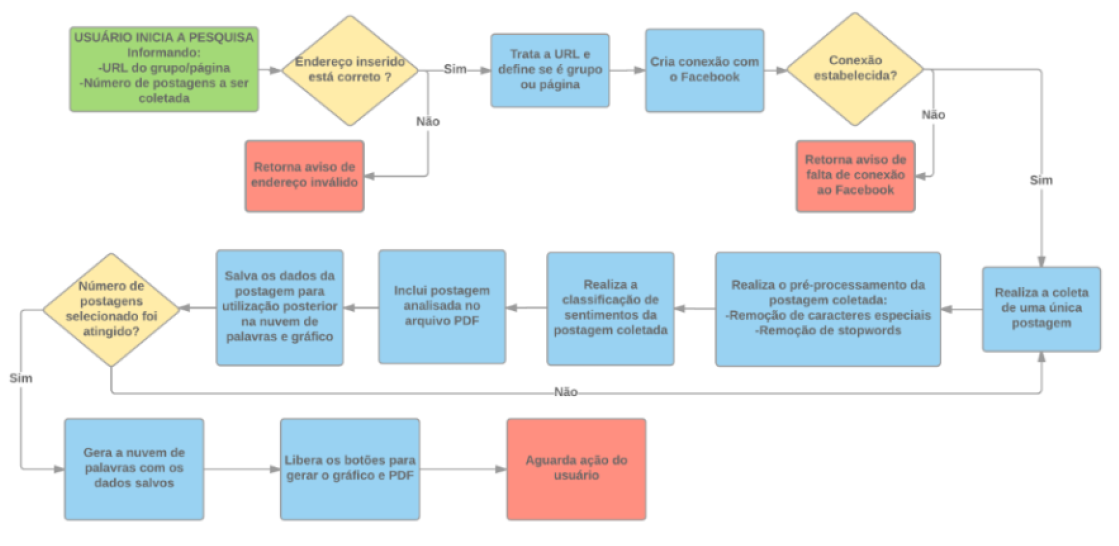
\includegraphics[scale=0.40]{imagens/fluxofilipe.png}
\legend{Fonte: \citeauthor{tccfilipe}}
\label{fig:fluxotccfilipe}
\end{figure}

\begin{figure}[!h]
\centering 
\caption{Menu de busca do \textit{software} revisado}
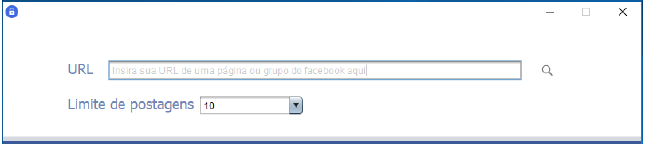
\includegraphics[scale=0.5]{imagens/menudebuscafilipe.png}
\legend{Fonte: \citeauthor{tccfilipe}}
\label{fig:menutccfilipe}
\end{figure}

\begin{figure}[!h]
\centering 
\caption{Nuvem de palavras do \textit{software} revisado}
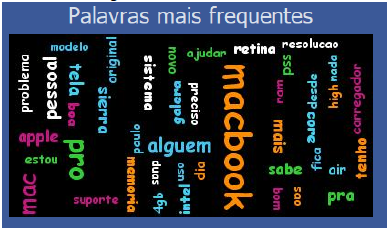
\includegraphics[scale=0.62]{imagens/nuvemdepalavras.png}
\legend{Fonte: \citeauthor{tccfilipe}}
\label{fig:nuvemtccfilipe}
\end{figure}

\begin{figure}[!h]
\centering 
\caption{Gráfico de sentimentos do \textit{software} revisado}
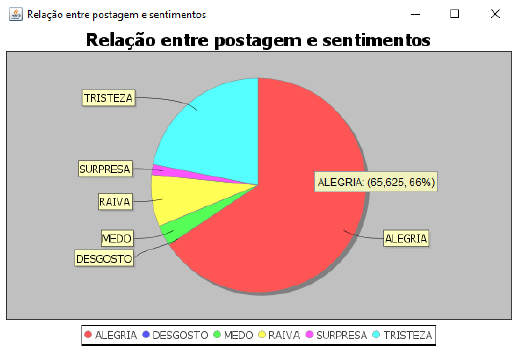
\includegraphics[scale=0.8]{imagens/graficodesentimentosfilipe.png}
\legend{Fonte: \citeauthor{tccfilipe}}
\label{fig:graficotccfilipe}
\end{figure}

\begin{figure}[!h]
\centering 
\caption{Resultado exportado do \textit{software} revisado}
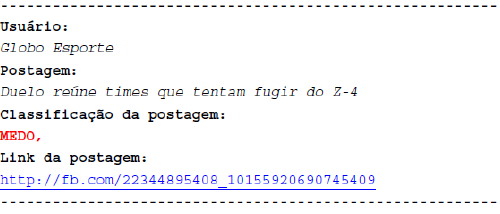
\includegraphics[scale=0.60]{imagens/exportadofilipe.png}
\legend{Fonte: \citeauthor{tccfilipe}}
\label{fig:exportadotccfilipe}
\end{figure}

\newpage
Para atingir o propósito de sua pesquisa, \citeonline{tccfilipe} realizou o estudo de léxicos de emoções contidos na base de dados chamada \textit{WordNet}\footnote{https://wordnet.princeton.edu} categorizados em seis grupos distintos que foram: alegria, desgosto, medo, raiva, surpresa e tristeza. Na Tabela \ref{tab:categoriaemo} estão alguns exemplos de palavras separadas pelas respectivas categorias de emoção selecionado pelo autor. Além da análise de sentimentos também foi implementada busca por palavras frequentemente encontradas em ataques de \textit{phishing},  e também palavras de linguagem imprópria, visto que as redes sociais não mantém um filtro de conteúdo levando em consideração a idade do usuário.

\begin{table}[h!]
  \begin{center}
    \caption{Categorias de emoções}
    \label{tab:categoriaemo}
    \begin{tabular}{ll} % <-- Alignments: 1st column left, 2nd middle and 3rd right, with vertical lines in between
      \textbf{Categoria} & \textbf{Palavras}\\
      \hline
      Alegria&animação, ânimo, comédia\\
      Desgosto&maldoso, chatear, abominável\\
      Medo&desespero, escuridão, friamente\\
      Raiva&assassinar, bravejar, detestar\\
      Surpresa&chocante, espanto, impressionado\\
      Tristeza&cabisbaixo, chorão, culpa\\
      \hline
    \end{tabular}
  \end{center}
  \legend{Fonte: \citeauthor{tccfilipe}}
\end{table}
Após definir os grupos de coleta, os dados de coleta para a análise de sentimentos e realizar a classificação dos dados utilizando método de classificação baseado em léxicos, o autor realizou a análise dos resultados para constatar o quão precisa foi a classificação realizada pela ferramenta. \citeonline{tccfilipe} coletou amostras de diferentes tamanhos em todos os grupos analisados totalizando 50 (cinquenta), 100 (cem) e 500 (quinhentos) postagens para, após, serem também analisadas manualmente e assim comparar os resultados. Dentre os grupos estudados estão a página do \textit{Outback Brasil} e o grupo da Previdência Social, alguns ajustes de léxicos foram necessários para que as classificações ocorressem com maior assertividade nos casos de alegria e tristeza. No final foi realizada a comparação entre as classificações e exatificadas as suas respectivas taxas de acerto, a Tabela \ref{tab:taxaacerto} apresenta os resultados obtidos, com eles foi possível verificar que quatro dos sentimentos tiveram taxa de acerto superiores a oitenta por cento. Com o cálculo do desvio padrão foi possível constatar que nos sentimentos com menor classificação refletiam uma grande dispersão em torno da media populacional, resultado de expressões ambíguas e de duplo sentido.

\begin{table}[h!]
  \begin{center}
    \caption{Taxa média de acerto na classificação de postagens analisadas}
    \label{tab:taxaacerto}
    \begin{tabular}{lllllll} % <-- Alignments: 1st column left, 2nd middle and 3rd right, with vertical lines in between
      \textbf{Classificação} & \textbf{Alegria} & \textbf{Medo} & \textbf{Tristeza} & \textbf{Desgosto} & \textbf{Raiva} & \textbf{Surpresa}\\
      \hline
      Taxa de Acerto&52,82\%&90,77\%&81,55\%&88,89\%&91,01\%&75,83\%\\
      Desvio Padrão($\sigma$)&16,06&2,62&5,20&4,61&4,23&9,97\\
      \hline
    \end{tabular}
  \end{center}
  \legend{Fonte: \citeauthor{tccfilipe}}
\end{table}

Ao final dos estudos foi concluído que a ferramenta desenvolvida trouxe resultados satisfatórios tanto pelos resultados obtidos como pela facilidade que a ferramenta desenvolvida trás para os usuários comuns. Ainda, foram apontadas melhorias para os estudos futuros entre elas o desenvolvimento de uma plataforma \textit{web}, aprimoramento nos testes de resultados da análise de sentimentos e também novas abordagens na etapa de classificação dos dados. 
% falar aqui sobre os resultados encontrados pelo filipe

\section{Integração com \textit{Software} Existente}
\label{sec:integracaosoftware}
Após a composição do \textit{corpus} com as palavras mais utilizadas em discursos de ódio, a nova etapa será agregar essa nova lista ao \textit{software} mencionado na Sessão \ref{sec:revisaoferramenta} para que o mesmo seja capaz de, além de identificar as seis categorias de emoção (alegria, desgosto, medo, raiva, surpresa e tristeza), identificar palavras impróprias e de possíveis ataques de \textit{phishing}, também identifique comentários de ódio comumente praticados pelos \textit{haters}.
Também será necessária a integração com o \textit{Twitter} por meio da API \textit{Twitter4J} já que o \textit{software} está integrado atualmente com o \textit{Facebook} (Figura \ref{fig:implementacao}). 

\begin{figure}[!h]
\centering 
\caption{Diagrama de integração \textit{software} existente}
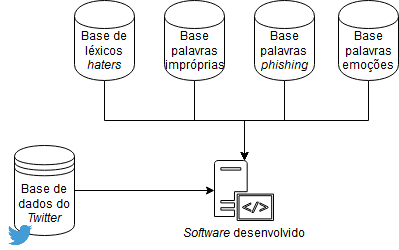
\includegraphics[scale=0.6]{imagens/implementacao.png}
\legend{Fonte: O Autor}
\label{fig:implementacao}
\end{figure}
Após a integração mencionada o trabalho atingirá seu objetivo geral e testes serão realizados para verificação de assertividade nas detecções de discursos de ódio dentre as subcategorias mencionadas na Sub-sessão \ref{subsec:classmanual}.

\section{Resultados Esperados}
Durante o desenvolvimento do trabalho, serão realizadas etapas que compõem a Análise de Sentimentos onde as mesmas serão aplicadas a um problema prático de detecção de discursos de ódio extraindo essas informações a partir de textos extraídos da rede social \textit{Twitter}.

Após a geração de base de dados rotulada manualmente por especialista humano a partir de amostras extraídas da rede mencionada, serão aplicados algoritmos supervisionados de classificação automática de textos e o de melhor desempenho irá auxiliar na composição de \textit{corpus} com as palavras mais frequentes em discursos de ódio. Com o \textit{software} integrado com novo \textit{corpus} pretende-se realizar testes com base aleatória de dados para realizar comparações e verificar a efetividade na detecção de discursos de ódio bem como a subcategoria que o texto compõe (discurso de raça, religião, gênero, incapacidade).
\chapter{Conclusões}
\label{cap:conclusoes}
Nesse capítulo serão apresentadas as conclusões obtidas na fase de desenvolvimento do Trabalho de Conclusão de Curso I. Uma síntese do trabalho realizado pode ser vista na Sessão \ref{sec:sintese}, já na Sessão \ref{sec:cronograma} poderá ser visto o cronograma atualizado para o desenvolvimento do TCC II, sendo esse realizado no segundo semestre de desenvolvimento.

\section{Síntese}
\label{sec:sintese}

Esse trabalho apresentou as principais etapas necessárias para a análise de sentimentos. Métodos de coleta de dados, pré-processamento e classificação automática dos dados, abordando os algoritmos e técnicas mais utilizadas nas literaturas recentes sobre o tema.

Também foi apresentado breve histórico sobre as redes sociais, o número de usuários e também os tipos de dados que cada uma das ferramentas aceitam. Para o trabalho desenvolvido foi escolhida a rede social \textit{Twitter} por ter textos sintetizados de até $280$ caracteres e porque a mesma tem uma grande quantidade de usuários no mundo todo.

Com os trabalhos relacionados foi possível verificar a importância de se desenvolver um dicionário de léxicos na língua portuguesa para casos de discurso de ódio já que é um problema presente na \textit{internet} e que poucos governos punem os \textit{haters} que o praticam.

O trabalho desenvolverá um dicionário de palavras da língua portuguesa utilizadas em discursos de ódio, coletando dados da rede social \textit{Twitter} e realizando o pré-processamento para diminuição de ruídos, e após, classificando com o \textit{software} \textit{Weka} usando os algoritmos \textit{Naive Bayes}, \textit{Bayse Net} e \textit{SVM}, escolhendo o de melhor acurácia conforme classificação manual realizada por especialista humano.

Ao final, será integrada essa nova funcionalidade em um \textit{software} desenvolvido por \citeonline{tccfilipe} em seu Trabalho de Conclusão de Curso. Testes de acurácia serão igualmente realizados para verificar se ferramenta é capaz de identificar discursos de ódio na língua portuguesa e ainda, dizer se é um discurso de ódio contra raça, gênero, deficiência ou religião já que essas são as principais categorias de discurso de ódio segundo estudo realizado por \citeonline{Chetty2018}.

\section{Cronograma para TCC II}
\label{sec:cronograma}

O cronograma do trabalho encontra-se na Tabela \ref{tab-cronograma}, onde as etapas são:

\begin{enumerate}
\item Coleta de dados no \textit{Twitter};
\item Montagem de base rotulada com especialista humano;
\item Aplicação de algoritmos de pré-processamento;
\item Aplicação de algoritmos de \textit{machine learning} no \textit{Weka} (NB, BN, SVM);
\item Geração de base de léxicos em português;
\item Testes com resultados;
\item Contribuições e trabalhos futuros;

\end{enumerate}

\begin{table}[h!]\begin{center}
	\caption{Cronograma}\label{tab-cronograma}
	\begin{tabular*}{\textwidth}{@{\extracolsep{\fill}} c c c c c c c}
		\toprule
		& Etapa & mar. & abr. & maio & jun. & jul. &\\
		\midrule
		&   1   &   X  &      &      &      &      &\\
		&   2   &   X  &   X  &      &      &      &\\
		&   3   &      &   X  &      &      &      &\\
		&   4   &      &   X  &   X  &      &      &\\
		&   5   &      &      &   X  &      &      &\\
		&   6   &      &      &   X  &      &      &\\
		&   6   &      &      &      &  X   &  X   &\\
		\bottomrule                             
	\end{tabular*}
\end{center}\end{table}

% \include{capitulos/4-metodologia}
%\include{capitulos/3-deteccao-doencas}
%\include{capitulos/4-svm}

% ----------------------------------------------------------
% RESULTADOS
% ----------------------------------------------------------
%\part{Proposta de solução}
%\include{capitulos/5-proposta}
%\include{capitulos/5-implementacao}
%\include{capitulos/6-consideracoes}

% ----------------------------------------------------------
% RESULTADOS
% ----------------------------------------------------------
%\part{Resultados}

%\include{capitulos/capitulo1}

% ----------------------------------------------------------
% Finaliza a parte no bookmark do PDF
% para que se inicie o bookmark na raiz
% e adiciona espaço de parte no Sumário
% ----------------------------------------------------------
%\phantompart

% ---
% Conclusão (outro exemplo de capítulo sem numeração e presente no sumário)
% ---
%\chapter*[Conclusão]{Conclusão}
%\addcontentsline{toc}{chapter}{Conclusão}
% ---


% ----------------------------------------------------------
% ELEMENTOS PÓS-TEXTUAIS
% ----------------------------------------------------------
\postextual
% ----------------------------------------------------------

% ----------------------------------------------------------
% Referências bibliográficas
% ----------------------------------------------------------
\bibliographystyle{abntex2-alf}
\bibliography{tcc}

% ----------------------------------------------------------
% Glossário
% ----------------------------------------------------------
%
% Consulte o manual da classe abntex2 para orientações sobre o glossário.
%
%\glossary

% ----------------------------------------------------------
% Apêndices
% ----------------------------------------------------------

% ---
% Inicia os apêndices
% ---
%\include{diversos/apendices}
% ---


% ----------------------------------------------------------
% Anexos
% ----------------------------------------------------------
%\include{diversos/anexos}

%---------------------------------------------------------------------
% INDICE REMISSIVO
%---------------------------------------------------------------------
%\phantompart
%\printindex
%---------------------------------------------------------------------

\end{document}
